%!TEX root = ../../thesis.tex
\define{\chapterpath}{\allchapterspath/humanexperiment}
\define{\imgpath}{\chapterpath/img}

\chapter{Can humans learn from unlabeled interactions}
\label{chapter:humanexperiment}
\minitoc


In previous chapters, we defined a new challenge of interaction without pre-coordination for human-robot interaction scenario, which we called \emph{learning from unlabeled interaction frames}. But can human solve this problem in a human-human interaction scenarios?

In this chapter, we start by introducing the challenges related to such human-human experimental studies and present some related works. Then, we present our experimental setup that investigates how human negotiate a protocol of interaction when they can not rely on already share one. We took inspiration from the constraints inherent to human-robot interaction, such as restricted perception and communication abilities. The task is a joint construction task in which participants hold asymmetric roles, and can communicate only by pressing buttons of undefined meanings. Our experimental results show that participants manage to successfully interact and understand each other under such restricted interaction. They usually rely on stereotyped situations to synchronize their communication and intended meanings. We identified that some situations types are more recurrent and more easily understood than others. Based on our observations, we take some lessons that can be applied to human-robot interaction scenarios. Among them, we observed that participants generated interpretation hypothesis of the communicative signals and tested their hypothesis on next events. This will be the basis for the development of following chapters. 

This work is a collaboration with Anna-Lisa Vollmer and Katharina J. Rohlfing.

%%%%%%%%%%%%%%%%%%%%%%%%%%%%%%%%%%%%%%%%%%%%%%
%%%%%%%%%%%%%%%%%%%%%%%%%%%%%%%%%%%%%%%%%%%%%%
%%%%%%%%%%%%%%%%%%%%%%%%%%%%%%%%%%%%%%%%%%%%%%
%%%%%%%%%%%%%%%%%%%%%%%%%%%%%%%%%%%%%%%%%%%%%%
%%%%%%%%%%%%%%%%%%%%%%%%%%%%%%%%%%%%%%%%%%%%%%
\section{Introduction}

\question{Studying the Co-Construction of Interaction Protocols \\ in Collaborative Tasks with Humans}

We consider the overall goal of developing a robot system which should learn from and interact with non-expert users. Without assuming that the robot understands human feedback (i.e., without programming the information on how and when feedback is given into the system beforehand) how should the system understand what the signals it perceives mean and what they are referring to (cf. Gavagai problem \cite{quine1964word})?

In interaction, humans align and effortlessly, maybe even automatically, create common ground in communication \cite{clark1991grounding,pickering2004toward}. For this, they dispose of an immense amount of shared information. They make use of frames established in the history of interaction. Frames create a common ground about the purpose of the interaction \cite{tomasello2009cultural,rohlfing2013learning} and include ``predictable, recurrent interactive structures'' (\cite{ninio1996pragmatic}, p. 171). Frames thus provide interactants with guidelines about how to behave (a protocol for interaction) and also help interactants to understand the communicative intentions of their interaction partner. It further comprise basic behavioral patterns like roles, turns, timing, and exchange mechanisms. We aim at investigating how these interaction protocols emerge, because it would shed light on the basic mechanisms underlying interaction and inform us about what are the main issues in building robots capable of a similar interactional flexibility as the one humans possess. We are for instance interested in what kind of strategies humans use to align and what kind of meanings of social signals they converge to. Therefore we need to conduct research into how interaction protocols are negotiated in human-human interaction, aiming for that the obtained findings could be used as priors for a robotic system interacting with humans.

Unlike humans, who assume an immense amount of shared information, a robot system cannot rely on already established protocols for interacting. This is because, on the one hand, little is known about the universal interaction protocols humans rely on in communication, and on the other hand, human-robot interaction (HRI) is still very different from human-human interaction, as it is clearly characterized by asymmetry and restrictiveness in the sense that the human and the robot in general do not have the same abilities, modalities, mechanisms, and body for communication, perception and action \cite{lohse2010investigating}. For example, a robot that does not have arms cannot gesture, a robot without the respective algorithms or sensors does not perceive gaze direction or understand speech commands, and without any knowledge of internal computational mechanisms it is difficult to assess how a robot perceives its interaction partner and his/her actions. It is thus important that robots are able to negotiate meaning online with their interaction partners.

We designed an experimental setup with which we aim at investigating the processes used by humans to negotiate a protocol of interaction, when they do not already share one. In this chapter, we present and justify the method used and mention the very results obtained from a pilot study employing the setup.

Humans and robots view the world differently, so if we want to transfer our results to human-robot interaction, we should not assume that in the interactions we want to investigate, the partners see the world/interaction in the same way. To investigate the process of negotiating an interaction protocol, we thus consider a setup of a joint construction task in which participants assume asymmetric roles: the role of a builder and the role of an architect. With building blocks, the builder should assemble a target structure which is unknown to him/her but which the architect knows. This collaborative construction task with a joint goal renders the communication between participants indispensable and thus the game is not solvable by either one of the participants alone, e.g. with mere exploration. Thus, failing to complete the game successfully is equivalent to failing to communicate successfully. Communication is not face-to-face but channels are restricted, so that it is not possible for participants to communicate via familiar verbal or non-verbal communication channels, as for example speech or gestures. At the same time, the setup does not constrain all aspects of communication and thereby gives participants much freedom with respect to some features, including timing and rhythm or possible meanings (e.g. of button presses). The setup does not impose a predefined sequence of interaction upon participants, as it is often done in HRI scenarios \cite{akgun12hri}, but still benefits from a laboratory setting in which we do not need to take the full complexity of natural social interaction into account. With the aim to simulate the sending of signals to an interaction partner who does not have the same perceptual capabilities -- similar as in an interaction with a robot -- in our study the architect does not know how exactly his/her signals are perceived by the builder. For the successful completion of the thus highly challenging joint task of the game, both participants have to learn how to interact with each other.

The main contribution of this chapter is the presentation of the novel experimental method of our study. We would like to demonstrate that it allows to study important questions for the understanding of human negotiation of interaction protocols in joint construction tasks and that these questions are very important for HRI in the long-term. We first briefly discuss related work, then present our method, the results of the pilot study, and conclude by highlighting the implications of our results for human-robot interaction.

% We designed an experimental setup with which we aim at investigating the processes used by humans to negotiate a protocol of interaction used to solve a collaborative task, when they do not already share one. In the current paper, we present and justify the method used and mention the very first preliminary results obtained from a pilot study employing the setup. This research undertaking should inform us about what are the main issues in building robots capable of similar interactional flexibility. We are for instance interested in what kind of strategies humans use to align and what kind of meanings of social signals they converge to. Whereas, on the long run, the obtained findings could be used as priors for a robotic system interacting with humans, in an initial step, we first need to shed light on how interaction protocols are negotiated in \emph{restricted, asymmetric human-human interaction}. To our knowledge, there exists little research in the field of linguistics or pragmatics on this topic. To investigate this process of negotiation, we chose to design an experimental semiotics study which enables us to modify communication in the desired way, namely to restrict communication between participants who are assuming asymmetric roles. The field of experimental semiotics studies the emergence and evolution of communication systems \cite{galantucci2009experimental}. Here, instead of computer simulations as conducted by others (see \cite{cangelosi2002simulating,steels2012experiments}), controlled experiments in laboratory settings are designed to observe communication between participants who perform joint tasks. For instance, Galantucci et al. showed that pairs of participants performing a joint task could coordinate their behavior by agreeing on a symbol system \cite{galantucci2005experimental}.


% In our study, two people play a game in restricted, asymmetric communication conditions. For the task in the game, the communication between participants should be indispensable. Thus, it should not be solvable by either one of the participants alone, e.g. with mere exploration. Therefore, we designed the task to be a joint construction task with asymmetric roles: the role of a builder and the role of an architect. With building blocks, the builder should assemble a target structure which is unknown to him/her but which the architect knows. 
% Communication is not face-to-face but restricted, so that it is not possible for participants to communicate via familiar verbal or non-verbal communication channels, as for example speech or gestures. At the same time, the setup does not constrain all aspects of communication and thereby preserves a certain degree of naturalness in communication. It gives participants much freedom with respect to some features, including timing and rhythm or possible meanings (e.g. of button presses). The setup does not impose a predefined sequence of interaction upon participants, as it is often done in HRI scenarios \cite{akgun12hri}, but still benefits from a laboratory setting in which we do not need to take the full complexity of natural social interaction into account. With the aim to simulate sending feedback to an interaction partner who does not have the same perceptual capabilities -- similar as in an interaction with a robot --, in our study the architect does not know how exactly his/her feedback is perceived by the builder. For the successful completion of the thus highly challenging joint task of the game, both participants have to learn how to interact with each other. Thus, failing to complete the game successfully is equivalent to failing to communicate successfully.


% The main contribution of the current paper is the presentation of the novel experimental method of our study. We would like to demonstrate that it allows to study important questions for the understanding of human negotiation of interaction protocols in joint construction tasks and that these questions are very important for HRI in the long-term. Also, we report preliminary results of a first pilot run of the study. We first briefly discuss related work, then present our method and the preliminary results of the pilot study and close with a conclusion.

%%%%%%%%%%%%%%%%%%%%%%%%%%%%%%%%%%%%%%%%%%%%%%
%%%%%%%%%%%%%%%%%%%%%%%%%%%%%%%%%%%%%%%%%%%%%%
%%%%%%%%%%%%%%%%%%%%%%%%%%%%%%%%%%%%%%%%%%%%%%
%%%%%%%%%%%%%%%%%%%%%%%%%%%%%%%%%%%%%%%%%%%%%%
%%%%%%%%%%%%%%%%%%%%%%%%%%%%%%%%%%%%%%%%%%%%%%
\section{Related work}

% In this section, we will briefly discuss the most relevant related work, which lie in the field of experimental semiotics, and highlight the novelty of our proposed experimental method.

To our knowledge, there exists little research in the field of linguistics or pragmatics on this topic. To investigate this process of negotiation, we chose to design an experimental semiotics study which enables us to modify communication in the desired way, namely to restrict communication between participants who are assuming asymmetric roles.

The field of experimental semiotics studies the emergence and evolution of communication systems \cite{galantucci2009experimental}. Here, instead of computer simulations as conducted by others (see \cite{cangelosi2002simulating,steels2012experiments}), controlled experiments in laboratory settings are designed to observe communication between participants who perform joint tasks. For instance, Galantucci et al. showed that pairs of participants performing a joint task could coordinate their behavior by agreeing on a symbol system \cite{galantucci2005experimental}.

Most experimental semiotics studies developed to study joint action involve symmetric communication (cf. \cite{Galantucci2011experimental}).
Two studies which do consider asymmetric communication are the studies conducted by de Ruiter et al. \cite{de2010exploring} and Griffiths et al. \cite{griffiths2012bottom}. 

In their score- and round-based Tacit Communication Game, de Ruiter et al. investigated the cognitive processes responsible for the development and the recognition of new conventions by looking at reaction time. In a 3-by-3 grid world, two participants each manipulate a shape. For both of the shapes, the ``sender'' sees a target configuration. He/she first has to communicate the other player's target configuration to the other player, the ``receiver'', and second has to bring the own shape to his/her own respective target. De Ruiter et al. found that participants succeeded $83\%$ of the time and that the timing of movements is used to indicate a position. When comparing success rates for when the sender saw versus did not see the receiver's moves, the authors found that the game involves bidirectional communication and receiving information about the other player facilitates communication. The harder the communicative problem was, the more planning time was needed by both participants.

The setup of the study conducted by Griffiths et al. \cite{griffiths2012bottom} is more directly related to our setup. It is based on the alien world game setup by Morlino et al., in which in a square world shown on a computer screen, positions (left or right) and movements (shake horizontally or shake vertically) of 16 objects have to be explored via a mouse to maximize a score \cite{morlino2010developing}. It investigates the learning of categories, so the objects belonged to four categories which were defined by certain properties of the objects. Each category was associated with a target manipulation, i.e. shape and weight determined where an object should be positioned and how it should be moved. In the work by Griffiths et al. the learner could realize this task with the help of information given by a tutor who had prior knowledge about the categories the learner should explore. For this alteration, two players played the originally single player game simultaneously in separate rooms over a network connection. The computer screens in this setup additionally showed six buttons underneath the grid world. The tutor's communication to the learner consisted of the pressing and releasing of these six buttons using a keyboard. This was the only action the tutor could perform on the world. The authors found that tutors most commonly send feedback and guidance instructions to the learners. Negative feedback was given least often and its amount correlated with task failure. Learners who ignored less signals performed the task better.

The main, very important difference between the two asymmetric setups described above and our setup concerns the very nature of the task. Whereas in Griffiths et al.'s study the task is solvable with mere exploration, in our setup the input of the architect is essential. The latter is also the case in the study by de Ruiter et al., but in our setup no score is displayed to either of the players who in our case are not separate learner and tutor, or receiver and sender, but they solve the task together assuming the roles of a builder and an architect. Correspondingly, in our setup, the game does not include multiple episodes or rounds but it is continuous with the builder deciding when the task is completed and the game ends. The game of the study by de Ruiter et al. is based on fixed turns which is not the case with our game, where participants can act simultaneously and react directly upon each others conduct. By designing a continuous game without displaying a score, interaction remains natural (i.e., free) to a high degree. 

Another important difference which makes our setup novel regards the restriction of communicative channels. In contrast to the other two works, in our setup, the architect is not aware of how his/her actions are presented on the builder side and how they will be perceived. This renders the situation similar to human-robot interaction. This difference should also minimize the use of simple iconic feedback (as for example encoding the manipulation of horizontally shaking the object by alternately pressing one button to the right and one button to the left as reported by Griffiths et al.)

% final sentence about summarizing how our setup is novel: what are the benefits of doing it our way?
% - no score
% - no rounds, continuous
% - restricted communication
% - awareness about presentation of actions

%%%%%%%%%%%%%%%%%%%%%%%%%%%%%%%%%%%%%%%%%%%%%%
%%%%%%%%%%%%%%%%%%%%%%%%%%%%%%%%%%%%%%%%%%%%%%
%%%%%%%%%%%%%%%%%%%%%%%%%%%%%%%%%%%%%%%%%%%%%%
%%%%%%%%%%%%%%%%%%%%%%%%%%%%%%%%%%%%%%%%%%%%%%
%%%%%%%%%%%%%%%%%%%%%%%%%%%%%%%%%%%%%%%%%%%%%%
\section{The Collaborative Construction Game}

With the aim that improving our understanding of how humans negotiate protocols of interaction could provide hints on how robots could do it also, we designed a new experimental setup which allows to constraint the communication channels between two partners in asymmetric roles who should collaborate in order to achieve a joint construction task. We consider a joint construction where only one participant is aware of the targeted construction (the architect) while only the other has the ability to achieve it (the builder). The communication between partners is reduced to the use of symbolic events that the architect can send to the builder. Neither the architect nor the builder are given any a priori information on the meaning of the symbolic signals and should agree on the meaning of such signals by the mean of the construction task.

This section describes the details of the experimental setup, the participants we recruited, and the protocol used for running the study.

% The builder can send all kinds of non-verbal signals to the architect. Only one way of communication is really restricted. 

\subsection{Setup}

\begin{figure}[!htbp]
\centering
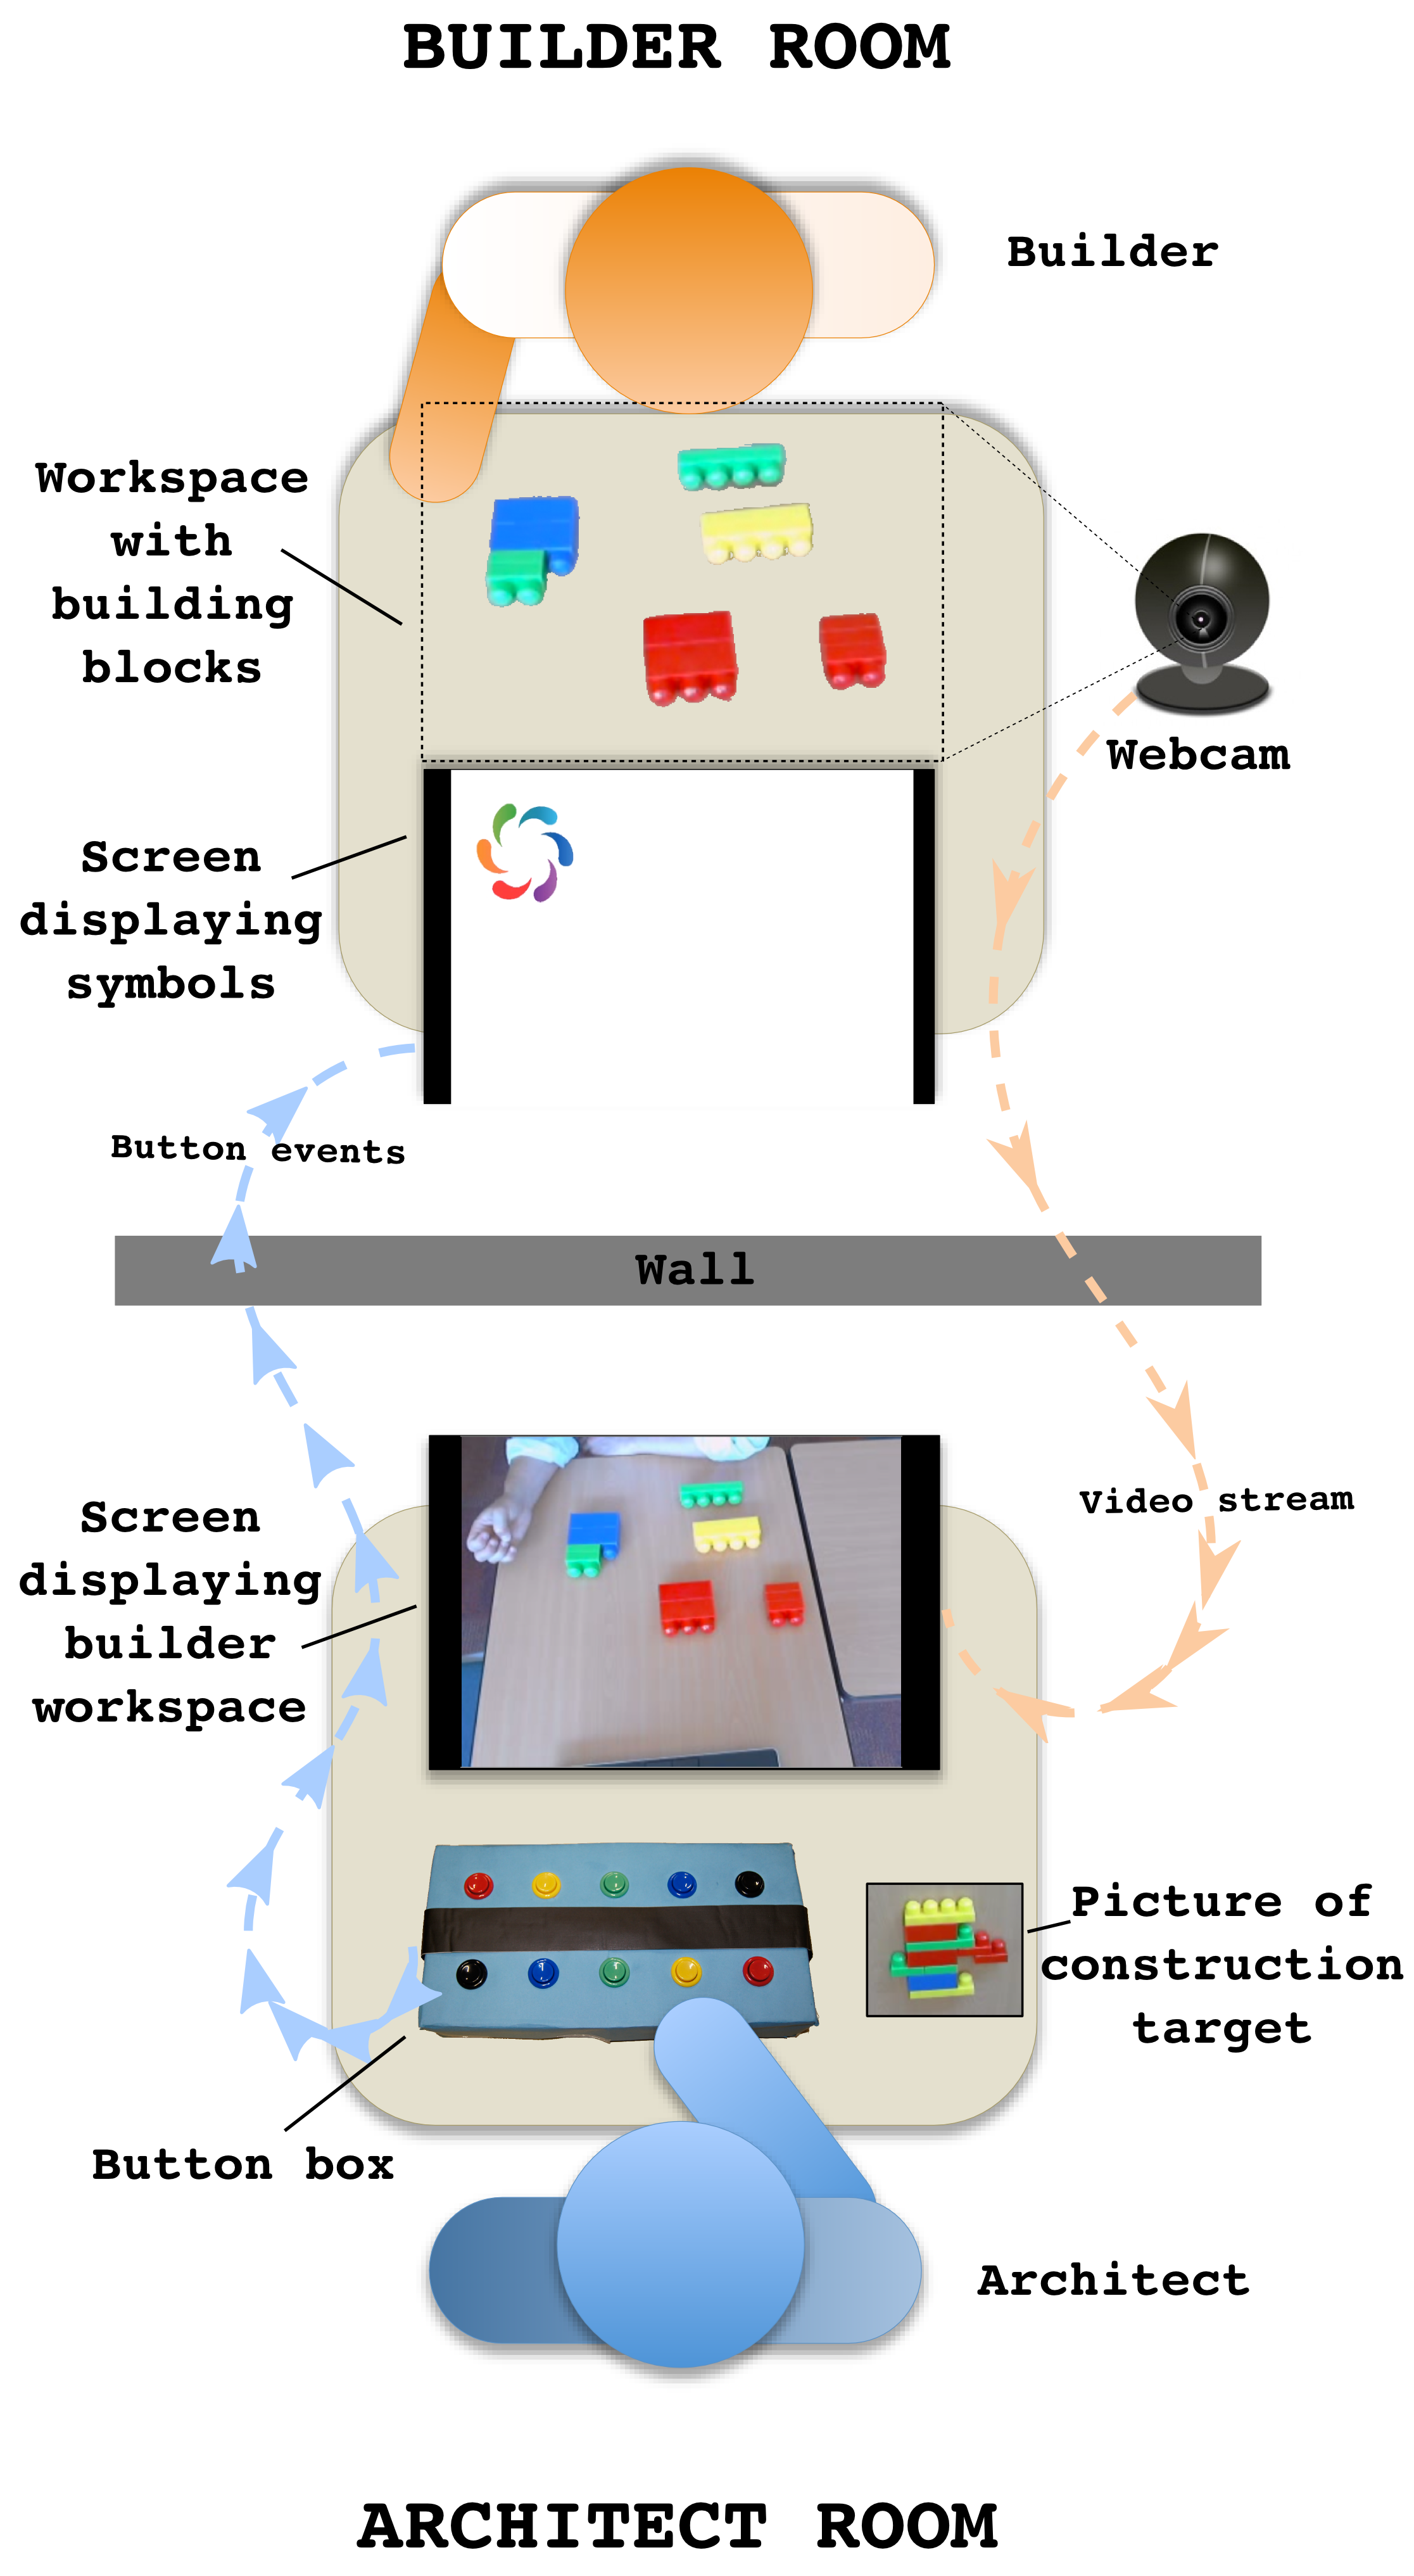
\includegraphics[width=0.68\columnwidth]{\visualspng/humanexp/setup/setup_normal_video_one_column.png}
\caption{Schematic view of our experimental setup. An architect (bottom) and a builder (top) should collaborate in order to build the construction target while located in different rooms. The architect has a picture of the targeted construction, while the builder has access to the construction blocks. The communication between them is restricted. The architect only sees a top view of the builder's workspace and can communicate with the builder only though the use of 10 buttons which, when pressed, display symbols on a screen on the builder side.}
\label{fig:overviewsetup}
\end{figure}

Figure~\ref{fig:overviewsetup} gives an overview of the experimental setup which considers an architect and a builder that are each seated at a table in front of a computer screen in two separate rooms and can neither hear nor see each other. 

The builder is equipped with a set of building blocks, in our case with 12 primary-colored Mega Bloks\textsuperscript{\textregistered} toy blocks differing in shape and color (see Figure~\ref{fig:bricks}). There were three red two-pads, two red three-pads, two yellow four-pads, two blue three-pads, two green two-pads, and one green four-pads blocks. 

The goal of the game is to assemble a specific construction yet unknown to the builder. As exemplified in Figure~\ref{fig:structures}, a construction is a flat combination of several blocks at least linked to one another by one pad. It does not necessarily contain all available blocks.

\begin{figure}[!htbp]
\centering
\begin{subfigure}[b]{0.49\columnwidth}
          \centering
          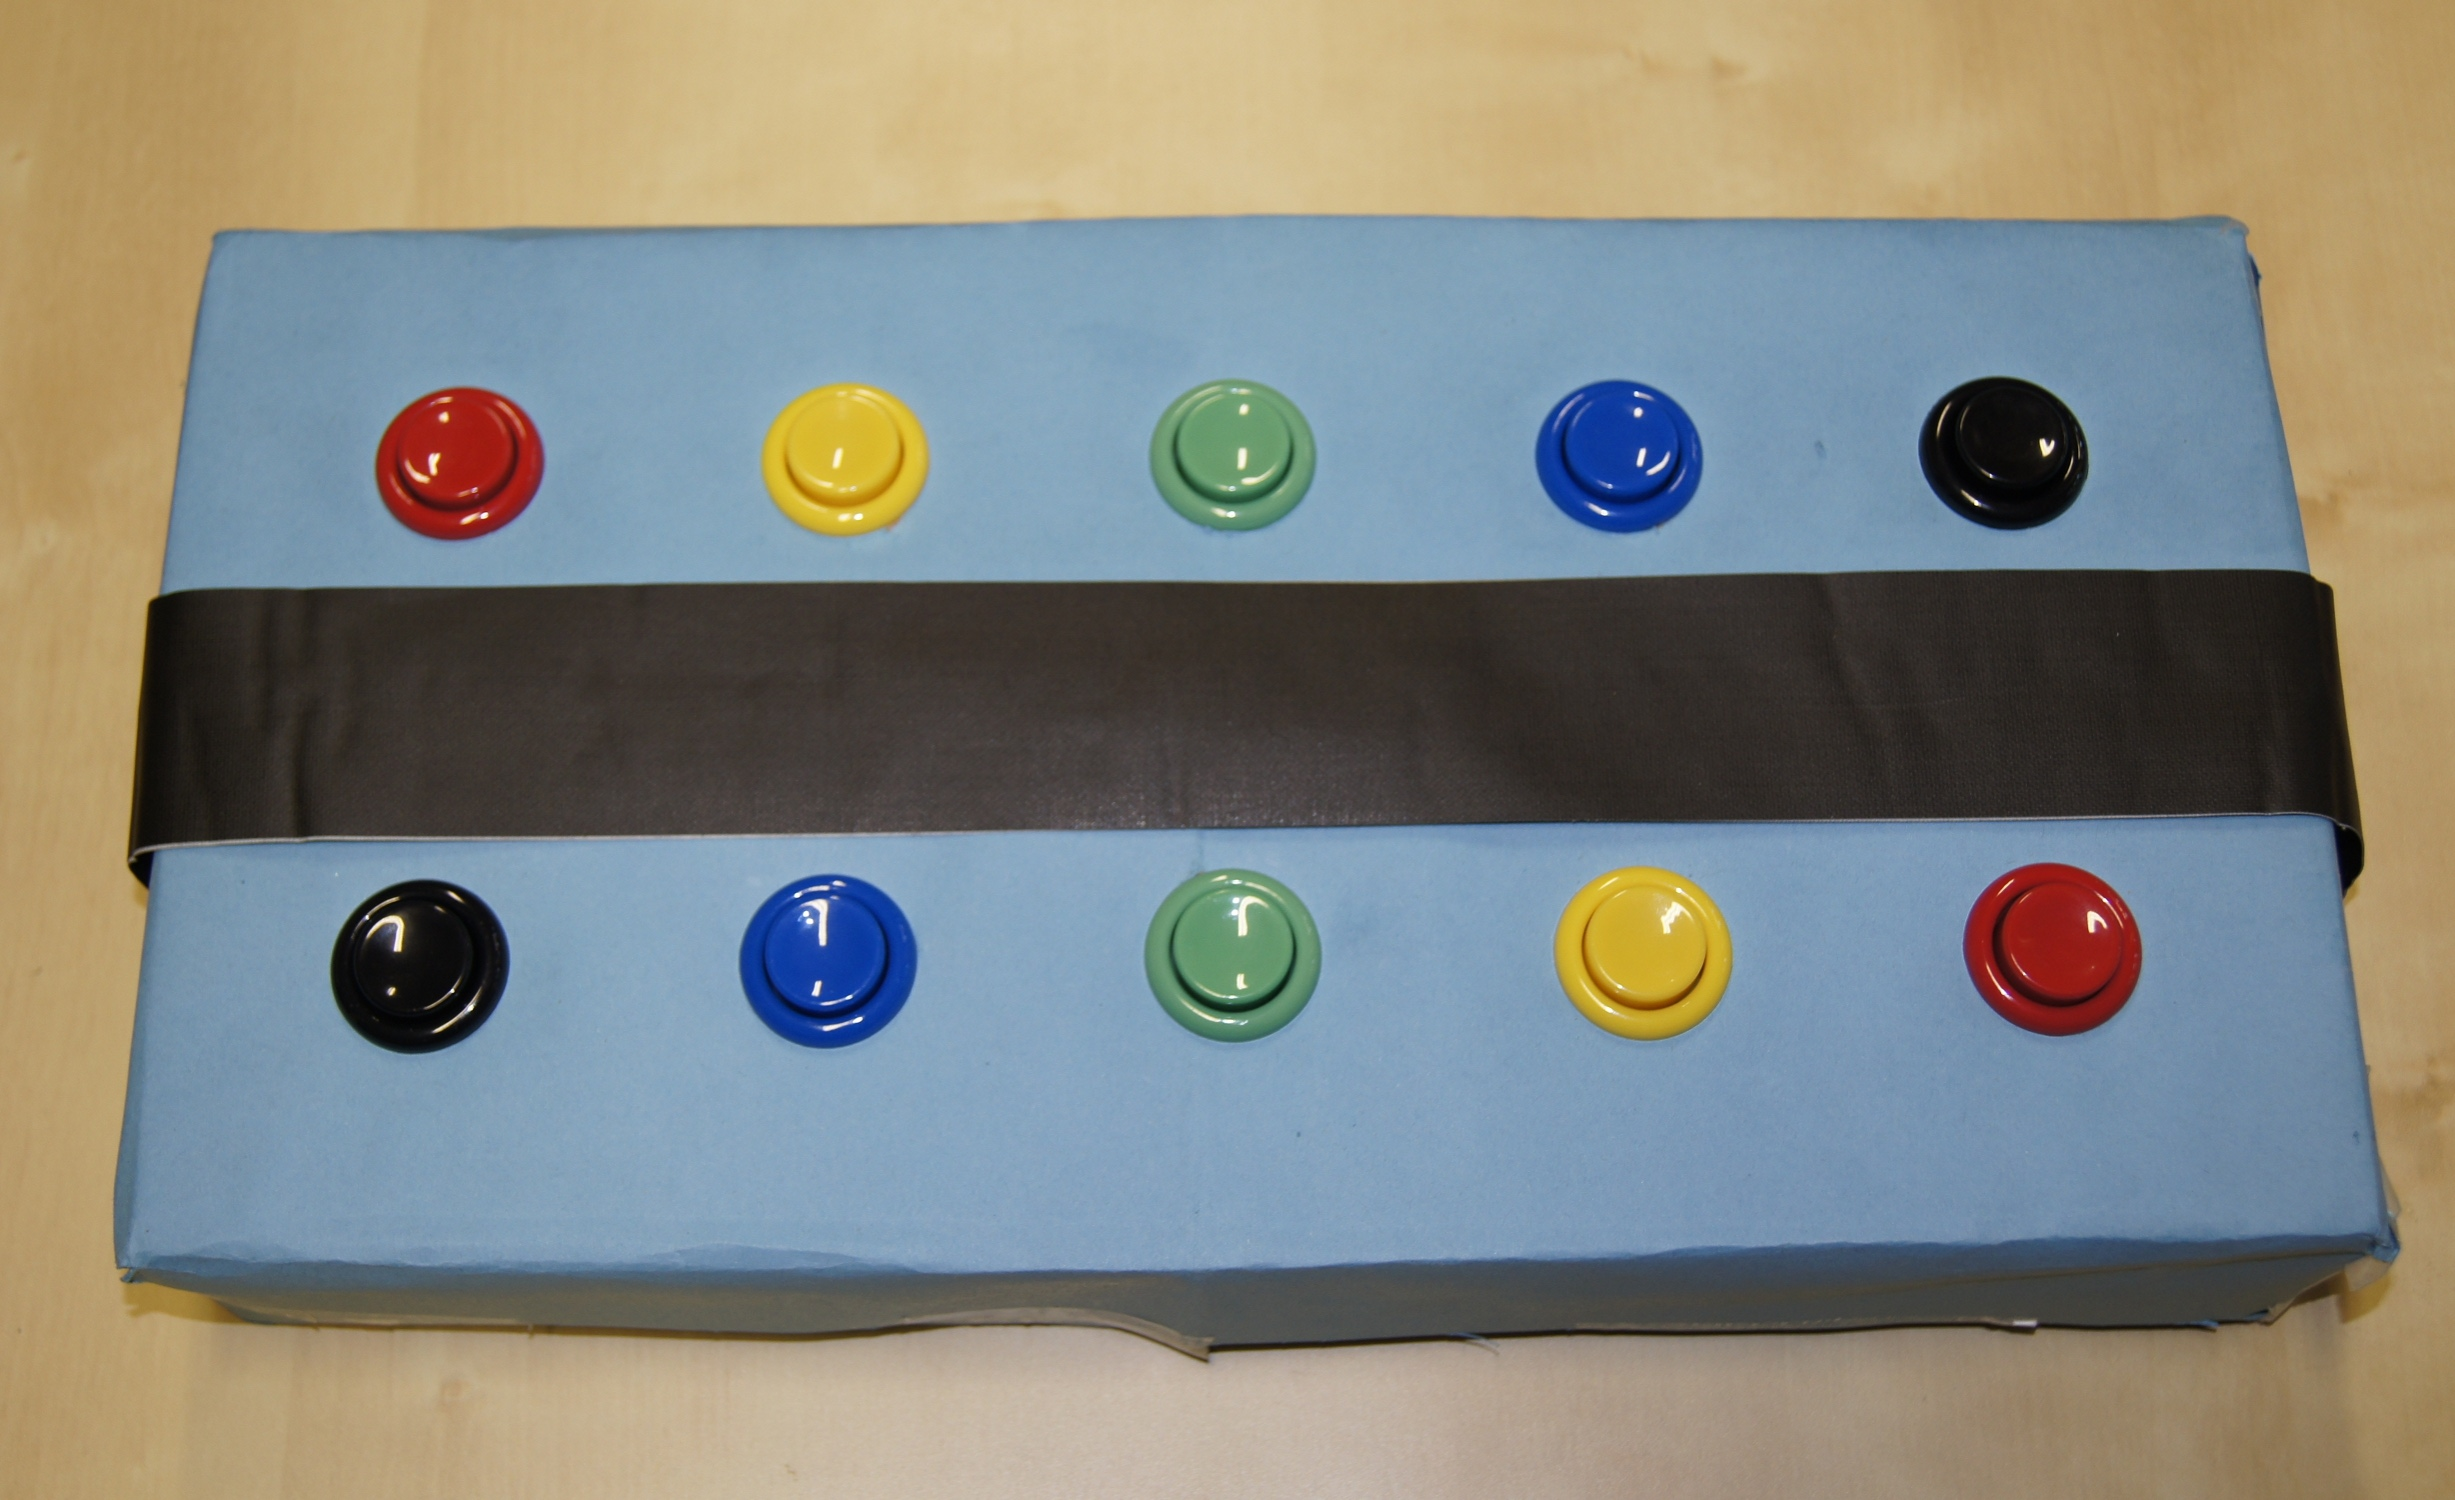
\includegraphics[height=3cm]{\imgpath/box.jpg}
          \caption{The box and the buttons used as an interface for the architect to communicate with the builder.}
          \label{fig:box}
\end{subfigure}
\begin{subfigure}[b]{0.49\columnwidth}
          \centering
          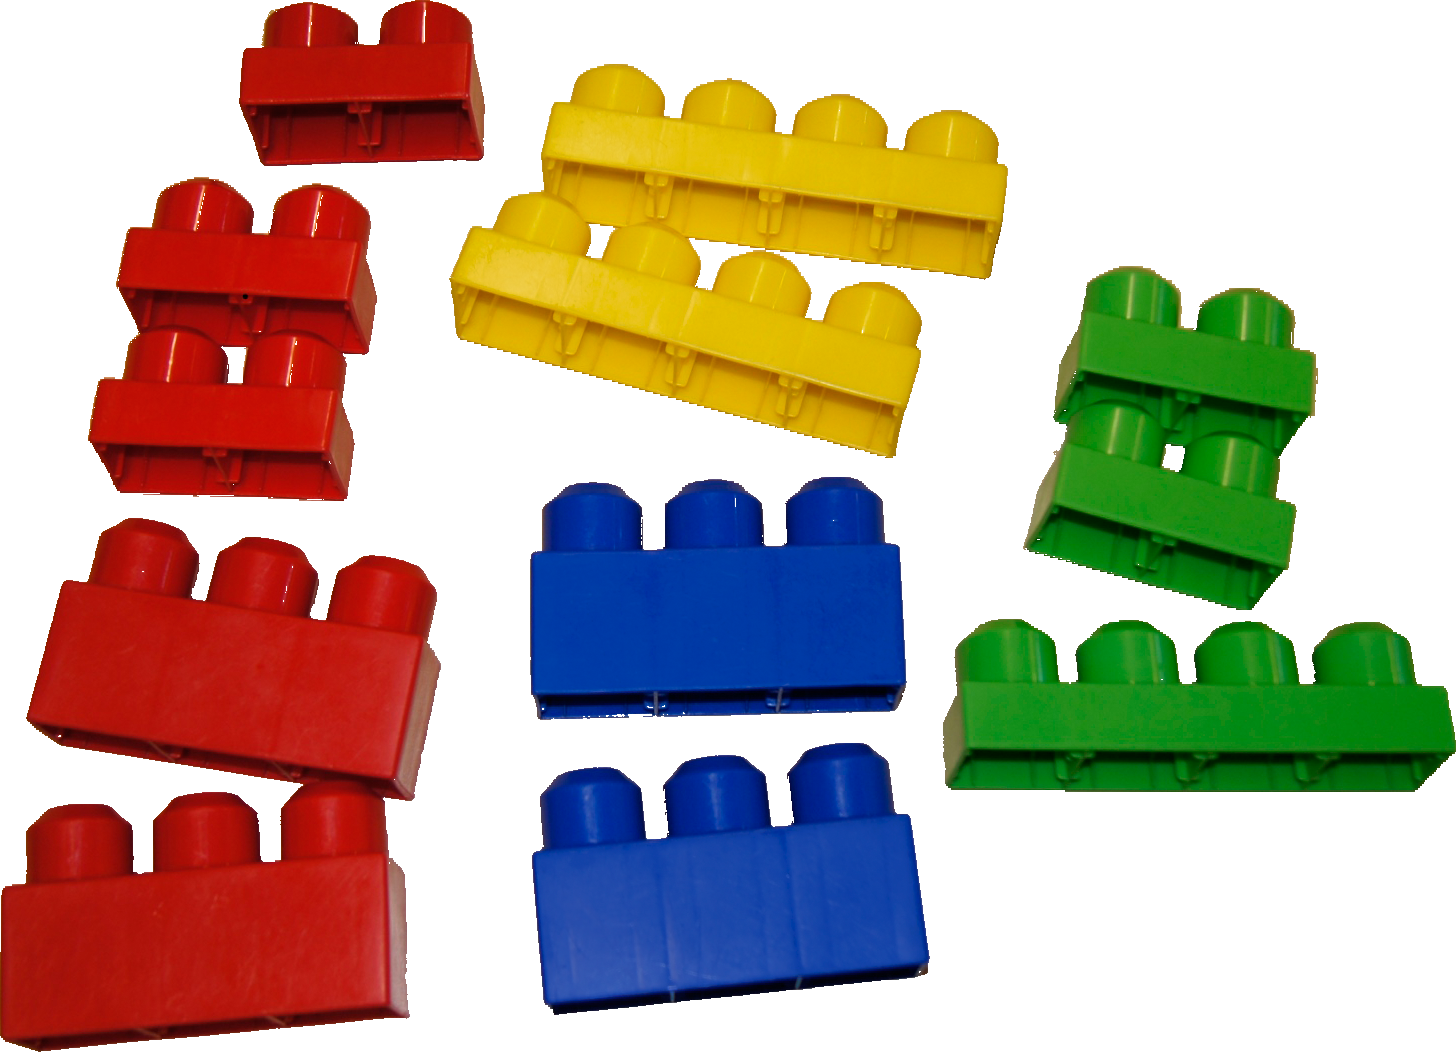
\includegraphics[height=3cm]{\imgpath/bricks.png}
          \caption{All toy blocks used in the collaborative construction task.}
          \label{fig:bricks}
\end{subfigure}
\caption{Elements of the setup.}
\label{fig:stuff}
\end{figure}

\begin{figure}[!htbp]
    \centering
    \begin{subfigure}[b]{0.24\columnwidth}
        \centering
        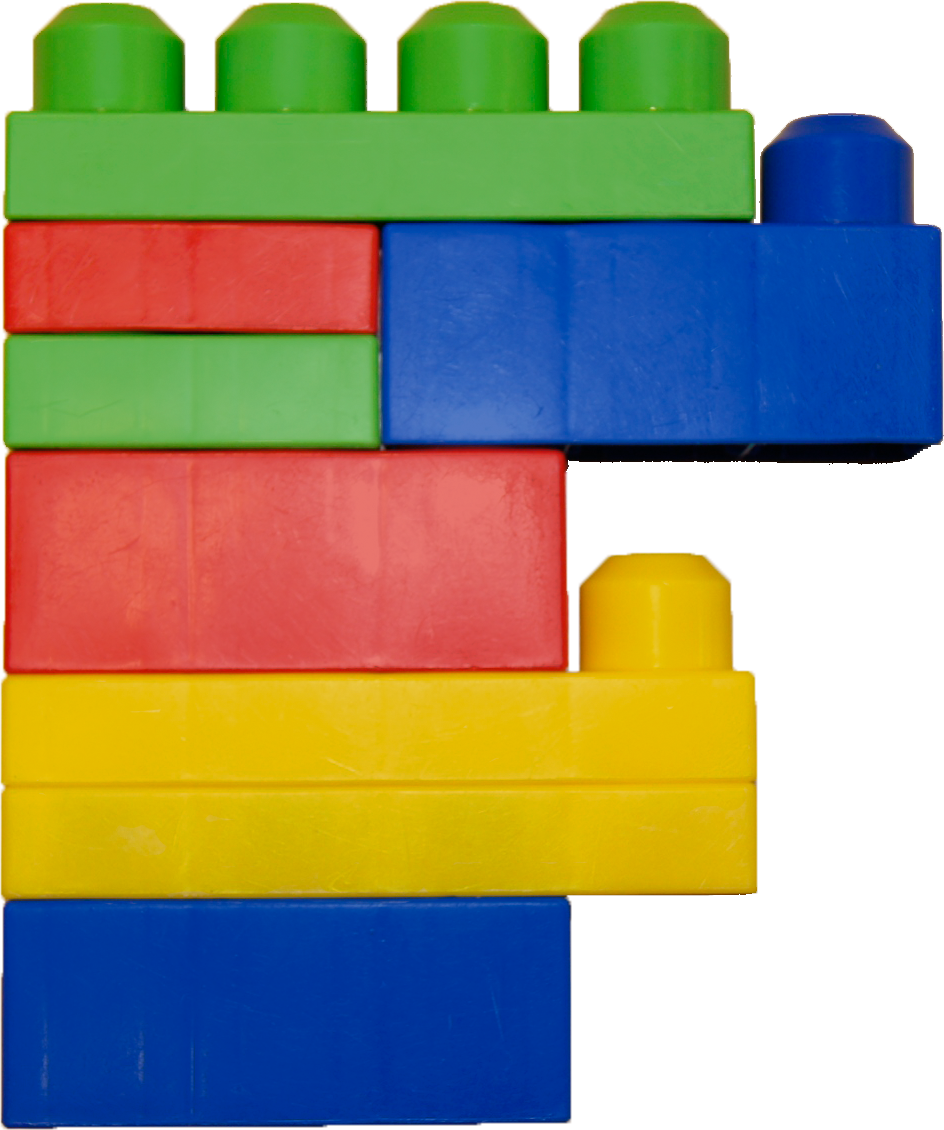
\includegraphics[height=3cm]{\imgpath/struct1.png}
        \caption{}
    \end{subfigure}
    \begin{subfigure}[b]{0.74\columnwidth}
        \centering
        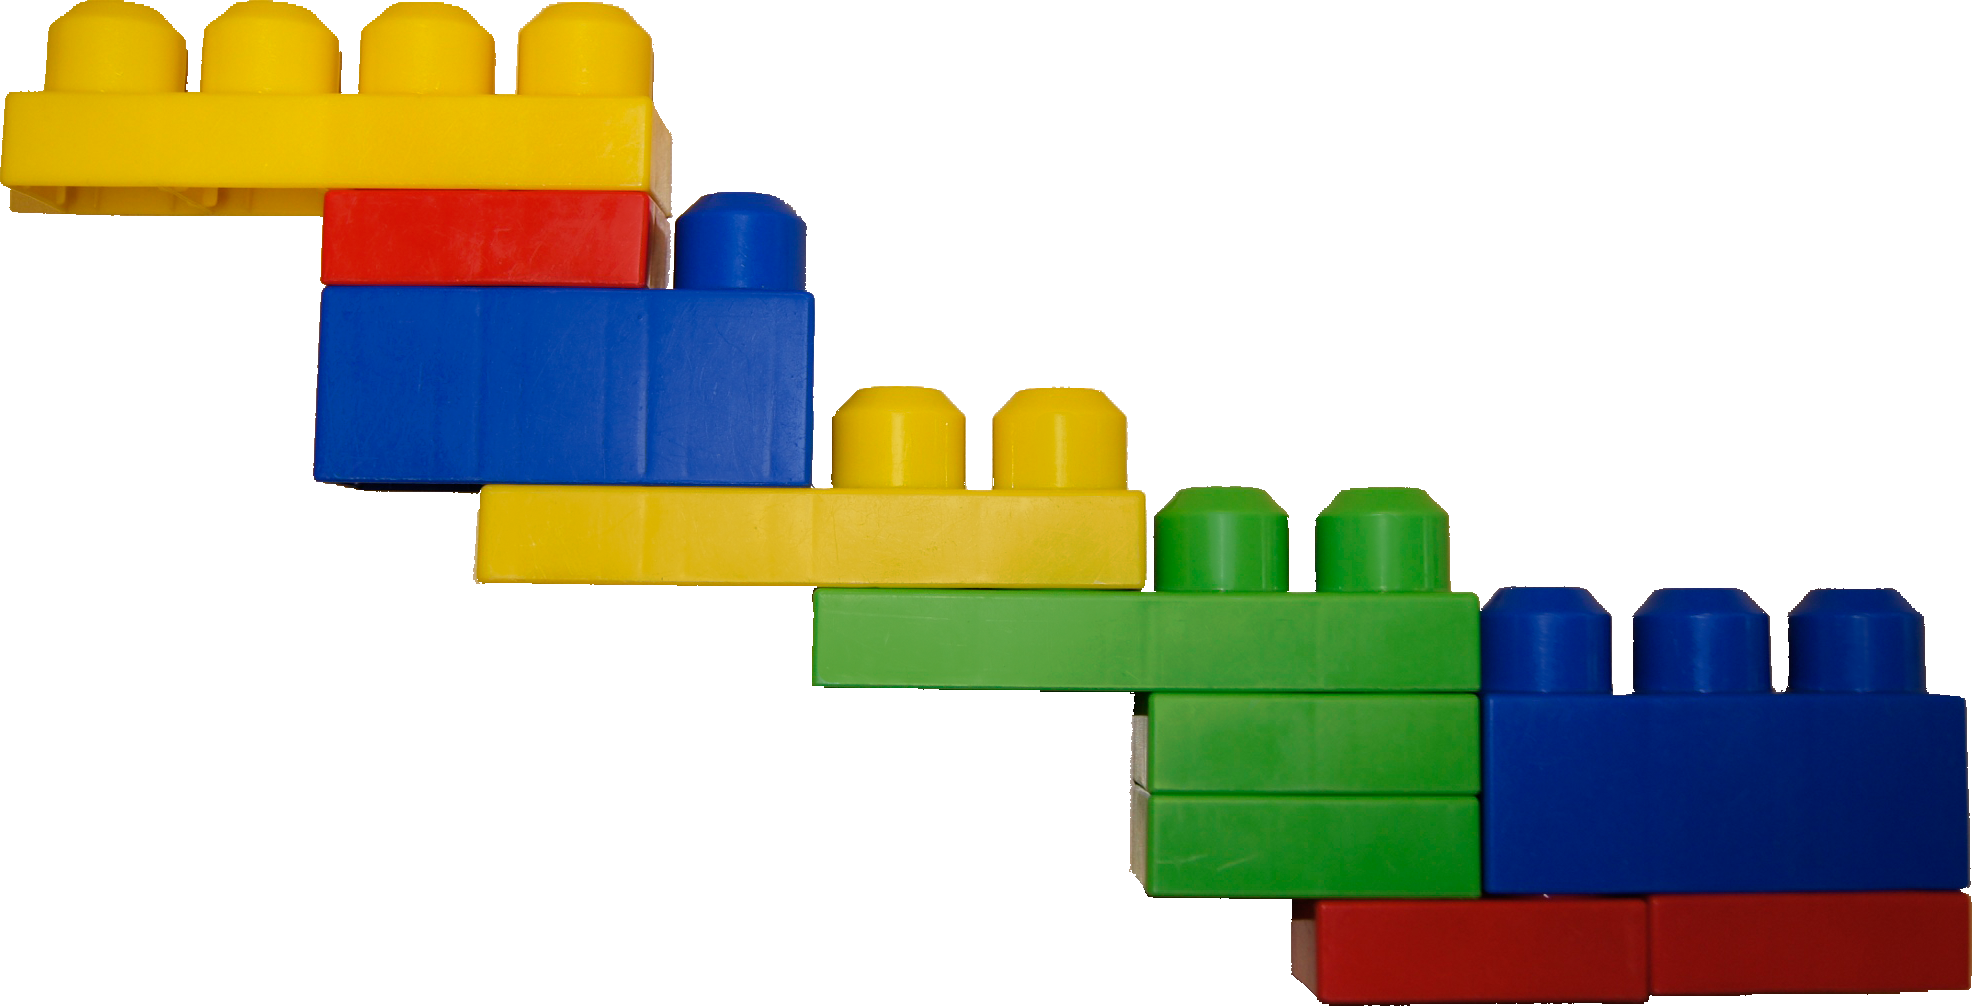
\includegraphics[height=3cm]{\imgpath/struct2.png}
        \caption{}
    \end{subfigure}
    \begin{subfigure}[b]{0.49\columnwidth}
        \centering
        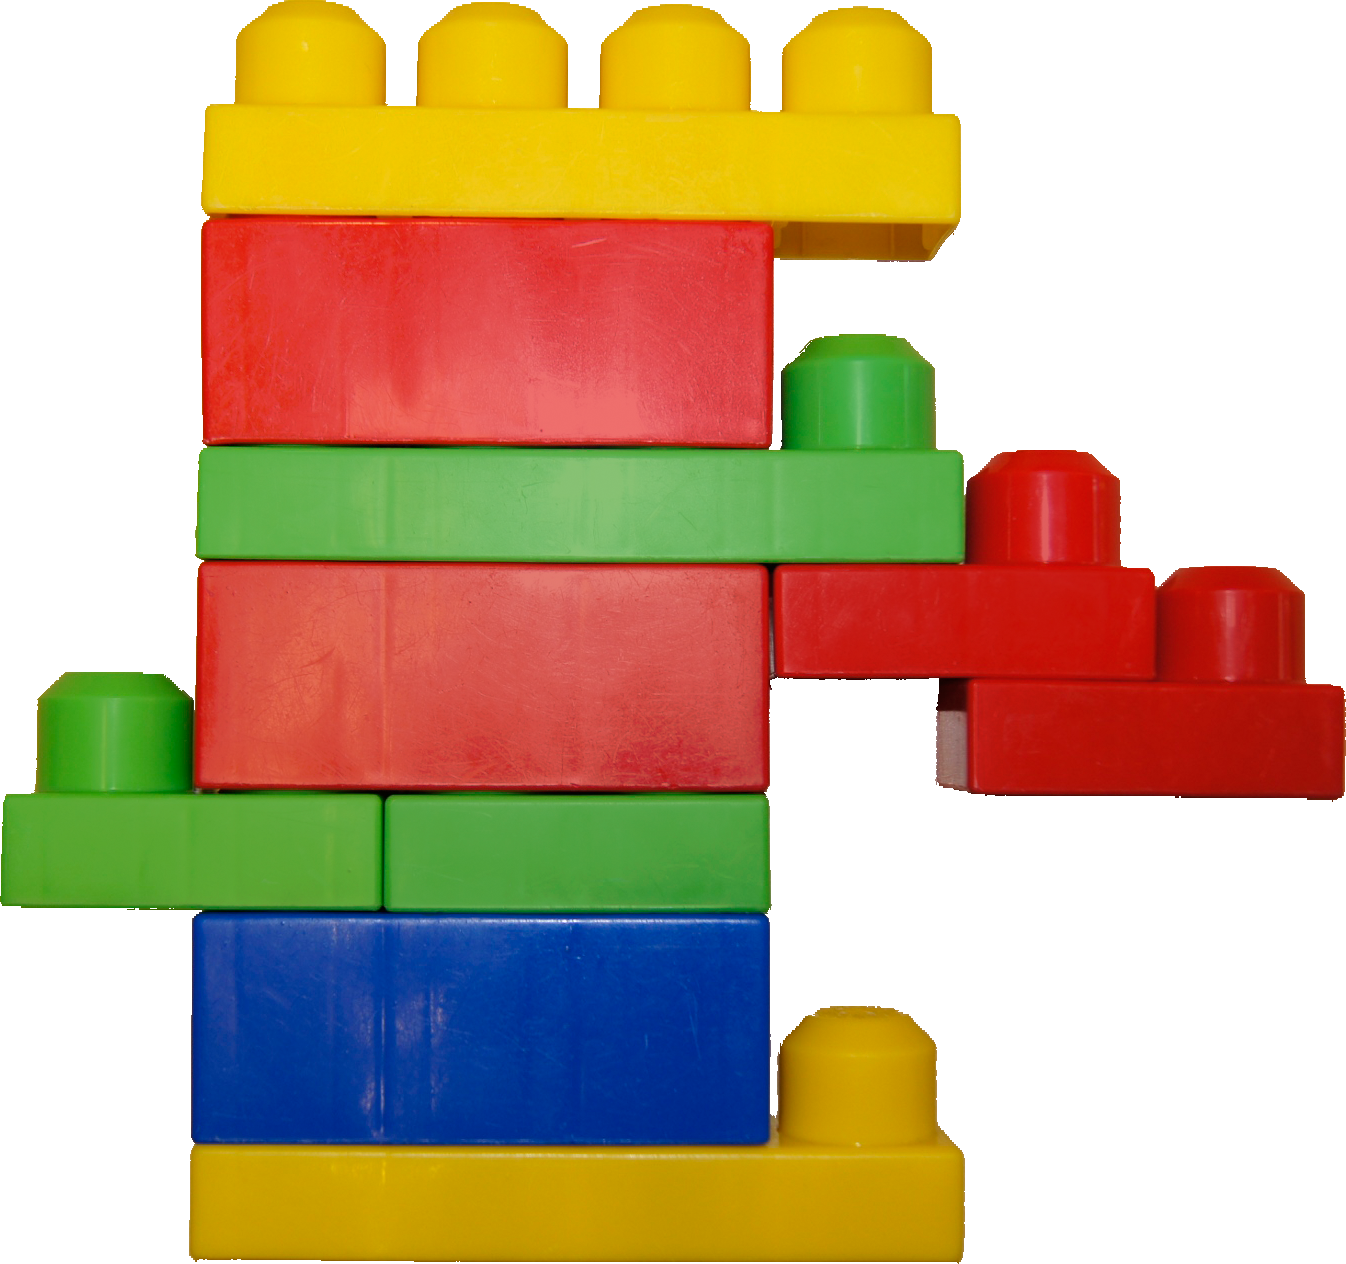
\includegraphics[height=3cm]{\imgpath/struct3.png}
        \caption{}
        \label{fig:sc}
    \end{subfigure}
    \begin{subfigure}[b]{0.49\columnwidth}
        \centering
        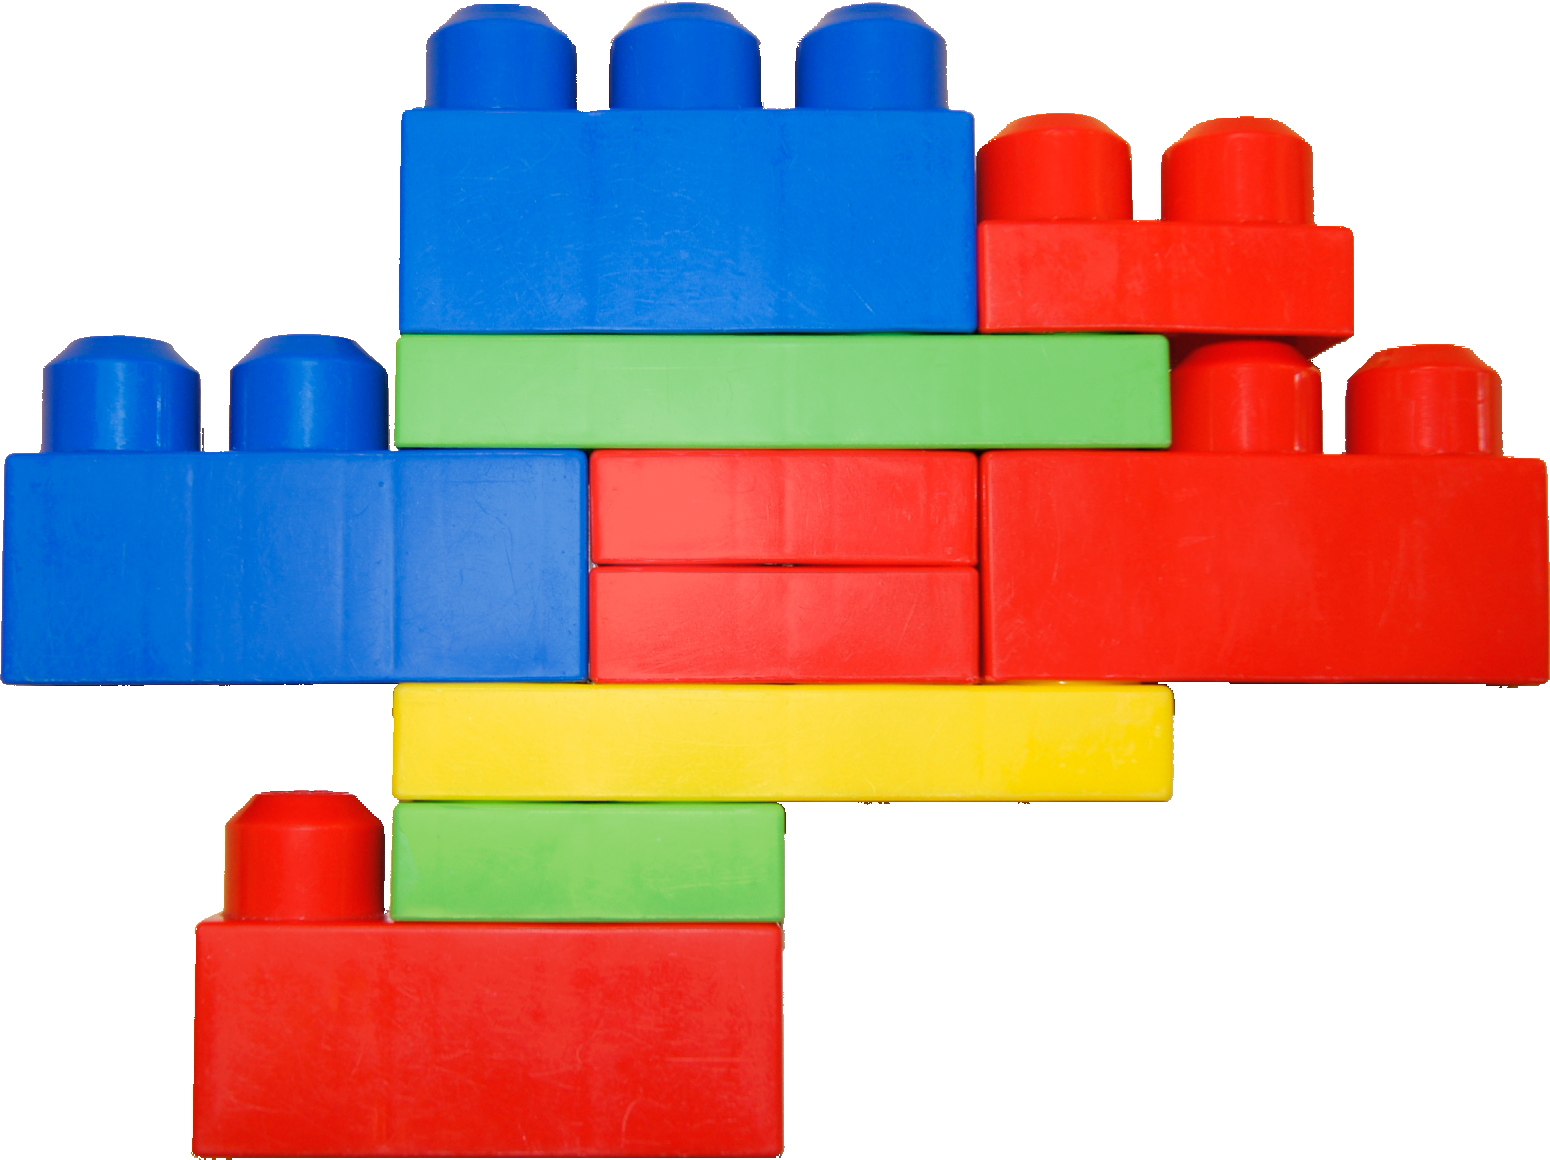
\includegraphics[height=3cm]{\imgpath/struct4.png}
        \caption{}
    \end{subfigure}
    \caption{Four examples of target structures presented to the architect.} 
    \label{fig:structures}
\end{figure}

The architect is given an image of the specific construction to be build and is told to guide the other player building it. A screen displays a live top view of the builder workspace. To communicate with the builder, the architect has access to a rudimentary interface made of 10 buttons, see Figure~\ref{fig:box}. Pressing a button displays a symbol on the screen located in the builder room. Each button is mapped to one of ten symbols and one of ten positions (two rows of five symbols) on the builder's screen, whereby the spacial organization of buttons differs from the spatial organization of displayed symbols. The mapping is randomized for each subject and fixed for the duration of one game. Figure~\ref{fig:sign} shows the different symbols.

\begin{figure}[!htbp]
\centering

\includegraphics[width=\columnwidth]{\visualspdf/humanexp/signs/signs.pdf}
\caption{The ten signs displayed on the builder screen.}
\label{fig:sign}
\end{figure}

\subsection{Participants}

We recruited 22 participants (19 m, 3 f) among students and staff at INRIA Bordeaux Sud-Ouest. Their age range was between 20 and 35 ($M = 25, SD = 3.91$) years. They played the collaborative game in pairs, where the two players in a pair were assigned randomly to the roles of a builder and an architect. Seven of the eleven pairs played the game together twice, such that each of the 14 participants involved assumed each role once. One second round of a dyad was excluded from the analyses, because the architect neglected the task instructions and altered the target structure during the game. This resulted in a total of 17 rounds.

\subsection{Procedure}
\label{sec:procedure}
Participants were not given the chance to talk about the game before it began. Architect and builder were instructed about their respective roles separately in their respective rooms. We presented the architects with a set of 20 pictures of different constructions from which they chose one. The builder was informed about the constraint that applied on the construction, i.e. flat construction which does not necessarily contain all available blocks. The architect and the builder were specifically told that the button positions did not directly map onto the symbols' positions displayed on the builder's screen, but that the mapping was fixed and arbitrary. Additionally, because the architect could see the hands of the builder during the game (see Figure~\ref{fig:overviewsetup}), the builder is told to only use his/her hands to move blocks and not to use hand signs. In practice, this was well respected by participants.

The game was \textbf{not} preceded by any training sessions. We aimed at reducing the time between the instruction of the participants and the beginning of the game as much as possible, so that they did not have time to elaborate any concrete strategy before the game began.

Once the game started, we observed the behavior of the two players and asked them to speak aloud about the meaning associated to the symbols/buttons. The experimenters took notes on the participants' remarks. The experiment stopped only when the builder decided and told the experimenters that the structure he had build was correct.

% During the experiments, the architects and builders were ask to speak aloud respectively what meaning they intended to convey by pressing a button and what they understood from the symbols displayed on the screen.

%%%%%%%%%%%%%%%%%%%%%%%%%%%%%%%%%%%%%%%%%%%%%%
%%%%%%%%%%%%%%%%%%%%%%%%%%%%%%%%%%%%%%%%%%%%%%
%%%%%%%%%%%%%%%%%%%%%%%%%%%%%%%%%%%%%%%%%%%%%%
%%%%%%%%%%%%%%%%%%%%%%%%%%%%%%%%%%%%%%%%%%%%%%
%%%%%%%%%%%%%%%%%%%%%%%%%%%%%%%%%%%%%%%%%%%%%%
\section{Results}

As stated before, the current pilot study serves as a proof of concept. We aimed at designing a setup allowing to study the processes involved in the formation of interaction protocols in asymmetric interaction with the particular constraint that the players could neither solve the task by themselves nor did they have access to any reward function.

Our pilot study revealed a great potential in the use of our experimental method to study many aspects of communication relevant to HRI. With our setup, we will be able to study, among others, questions related to alignment, rhythm, contingency, and feedback, which have been in the focus of HRI research for some time \cite{kopp2010social,michalowski2007dancing,fischer2013impact,vollmer2014robots,pitsch2013robot,wrede2010appropriate}.

Surprisingly, while the construction task in this setup seems really challenging on paper and participants thought they would never succeed, a majority of the architect-builder pairs succeeded on building the correct construction. We analyzed a total of 17 experiments, of which 13 were successful and 4 failed. The average duration of the runs was 18 minutes ($M = 18~min, SD = 11~min$) with a minimum of 7 minutes and a maximum of 45 minutes.

In what follows, we showcase results supporting our claim that our setup can be used to study the co-construction of meaning in restricted, asymmetric interaction. We will first show one run of the game in detail which should give the reader an idea about what happens during an interaction and the richness and aptness of the data to consider a variety of research questions. Then, we will continue with presenting our results on the negotiation of signal meanings and with describing observations of the builder behavior. We will conclude with mentioning interesting additional considerations which are beyond the scope of this work.

\subsection{One experiment in detail} 
\label{sec:case}

Figure~\ref{fig:timeline} brings together information about button presses (logs), their intended and interpreted meanings (found by the experimenters from their notes and observations of logs), and the builder's actions (builder video of the construction workspace) and makes clear the bi-directionality of the interaction. On the bottom of the figure, we see that the builder proposes blocks to the architect (blocks not belonging to the target structure in black, blocks belonging to it in gray) (cf. Subsection~\ref{sec:builder}) and on the top we see how the architect responds to the builder's actions in terms of button presses and meanings. Additionally, we see how the builder interprets these signals of button presses which he/she perceives as symbols on a screen (middle timeline of button presses and meanings) and how these interpretations and believes in turn again influence what the builder does next.

\begin{figure}[!htbp]
\begin{widepage}
\centering
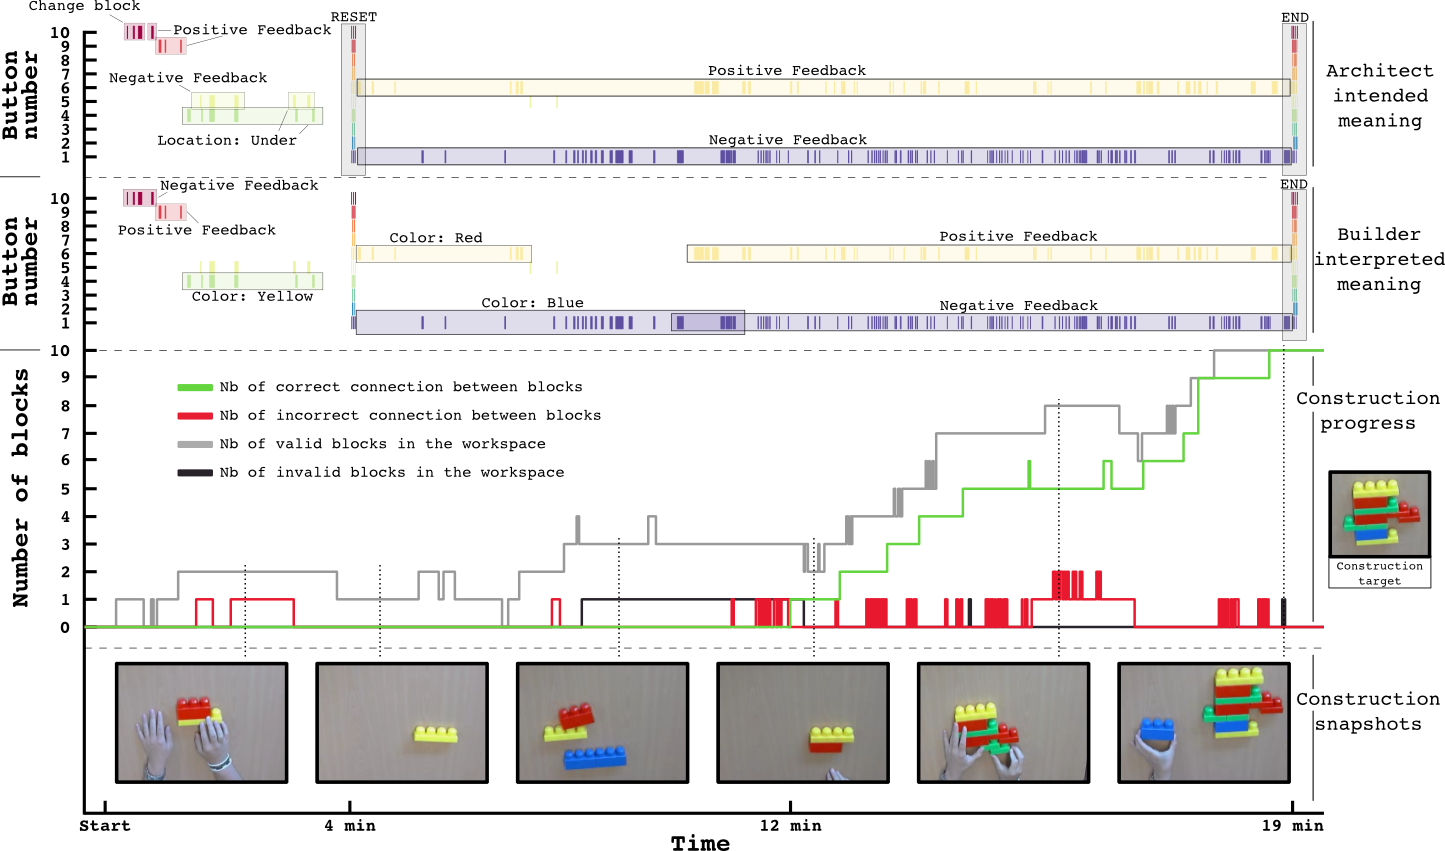
\includegraphics[width=1\textwidth]{\visualspng/humanexp/timeline/timeline_with_visu.png}
\end{widepage}
\caption{Timeline for one experiment of an architect and a builder collaborating towards building the construction target (right hand side). The top and middle part show the timeline of button presses associated with the intended meaning from the architect (top) and the understood meaning from the builder (middle). There were 10 buttons, for which we logged all button presses for each experiment and here display all occurrences as colored dashes. The button events are annotated with the meaning the architect intended or the builder understood as participants reported during the game. Events that are not annotated were not mentioned by the participants. At the bottom, the figure additionally visualizes the progress made by the builder in assembling the target structure and also shows incorrect block propositions, joining of incorrect blocks and mistakes. These events were annotated by hand using the video annotation tool ELAN developed by the Max Planck Institute for Psycholinguistics, The Language Archive, Nijmegen, The Netherlands \cite{wittenburg2006elan}. A block proposition here started, when the transportation of the block towards the workspace ended and the block lay still on the table. It ended when the block was again picked up and subsequently removed from the workspace. These presentation events were classified into correct and incorrect propositions by determining whether the proposed block was part of the target structure. Equivalently, a joining event started when two blocks were successfully joined at either a correct or incorrect position (again depending on whether the resulting configuration was part of the target structure). It ended before right before the two previously joined blocks were again pulled apart.}
\label{fig:timeline}
\end{figure}

With respect to the meanings of the button presses, we observe changes of button meanings over the course of the interaction. The exact points in time when meaning changes occur have been matched to the button presses by hand and is therefore approximated. While this may be a problem for detailed analyses on a micro level, it is of little importance for the macro analysis presented here. During the first 4 minutes, the architect changes the intended meanings of signals many times and these meanings were not aligned with the builder's interpretation of signals. At 4 minutes, the architect presses all buttons at once, seemingly attempting to ask the builder to clear his/her mind and start over again. Right after this \emph{Reset} signal, the architect changes to one simple \emph{yes/no} strategy using button 1 and 6. On the builder's end, this Reset signal is followed by a pause of actions which hints at a direct confusion. It is only at 12 minutes into the game that the builder fully understands the intended meaning of the architect's button presses and can start joining two blocks correctly (green graph on the bottom). The experiment continues with the builder suggesting new blocks (bottom - black and gray events) and positions for new blocks (bottom - red and green events) one at a time which are validated or invalidated by the architect. After 19 minutes, the architect presses again all the buttons but this time with the aim of informing the builder that the construction is complete. The builder ended the experiment at that time. The \emph{End} signal was well interpreted by the builder as the interaction was going smoothly until that time and the few remaining blocks were rejected (bottom - black event at 19 min). The final construction was indeed the target one intended by the architect, hence resulting in a successful experiment.

Our setup allows to study the evolution of meanings associated to each button and put it in relation with the current context in the interaction. We find that the constraints inherent to our setup allow to analyze communication, especially the interplay of individual actions and their interactional history, as well as their concrete timing, while lowering interactional complexity and thereby reducing communicative noise.

\subsection{Meanings}

Architects and builders start the game without having agreed on specific meanings the buttons should convey. We start by studying the associated meanings obtained from our notes on signal meanings reported by builder and architect. They seemed to initially consider a large set of possible meanings, but, in the end, were able to agree primarily on only a limited number.

\paragraph{Types of Meanings} 

When analyzing the notes on the participants' explanation of signal meanings (see Subsection \ref{sec:procedure}), we identified nine different categories of meanings:

\begin{enumerate}
    \item \textbf{Positive Feedback}
    \item \textbf{Negative Feedback}
    \item \textbf{End}: The construction is finished.
    \item \textbf{Reset}: Start over.
    \item \textbf{Guidance}: Instruction on what to do. It includes \emph{change, invert, revert, new block, continue, stack}. 
    \item \textbf{Color}: Reference to the color of a block. It includes \emph{yellow, blue, red, green}.
    \item \textbf{Size}: Reference to the size of a block. It includes \emph{small, medium, big}.
    \item \textbf{Location}: Reference to the location of a block. It includes \emph{under, above, left, right}.
    \item \textbf{Group}: Reference to a group of blocks. It includes \emph{in, out, group\_X}.
\end{enumerate}

Importantly, those categories where \textbf{not} suggested to the participants beforehand, but only identified by us in a posteriori analysis.

For each experiment, we determined if the architect or the builder considered each type of meaning (see Figure~\ref{fig:types_of_feedback}). In every single experiment, positive and negative feedback were considered on both architect and builder side. The \emph{End} meaning has been considered on both sides in 14 experiments. More concrete instructions such as \emph{Guidance, Color, Size, or Location} were less often considered, especially by the builder.

\begin{figure}[!htbp]
  \begin{center}
      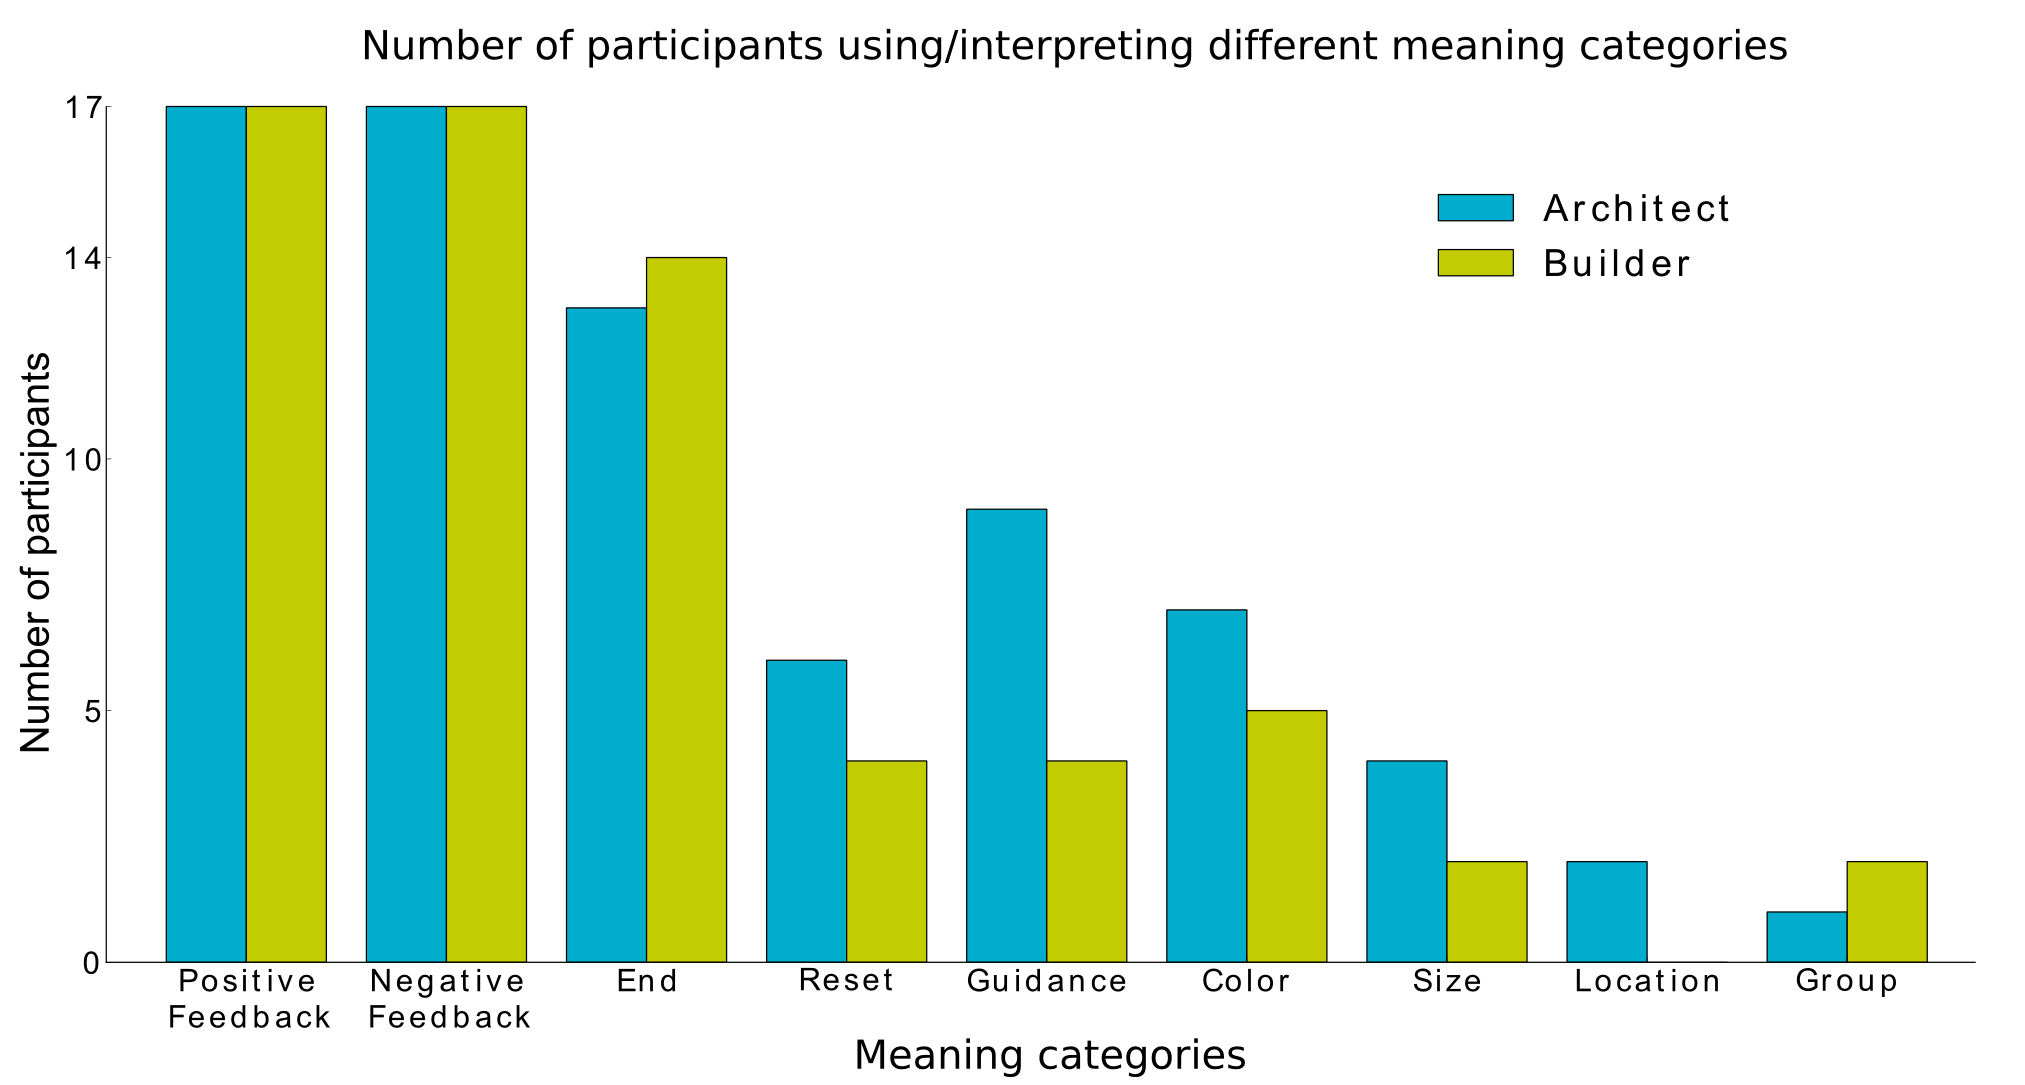
\includegraphics[width=\columnwidth]{\visualspdf/humanexp/meanings/instruction_type.pdf}
      \caption{Number of participants that used (architect) or interpreted (builder) signals as conveying different types of meaning. All participants considered positive and negative feedback.}
    \label{fig:types_of_feedback}
  \end{center}
\end{figure}

This is in line with the findings in \cite{griffiths2012bottom}, where ``correct'' and ``incorrect'' were also identified to be among the most common types of signal meanings.

\paragraph{Matching of meanings between architect and builder} 

Knowing which meaning categories were considered by each of the participants does not tell us if a particular pair of players understood each other. We therefore compared the associated meanings reported by architect and builder for all signals. Similarly to \cite{griffiths2012bottom}, we then determined the number of signals that were understood, misinterpreted, or ignored. We define signals which were understood as signals where both architect and builder agree on a common meaning. For signals which were misinterpreted, the builder reported a different associated meaning than the one intended by the architect. The signals which were mentioned by the architect, but not by the builder, were counted as ignored signals. We then averaged the results for successful and failed experiments, see figure~\ref{fig:types_of_understanding}. For successful experiments, the average number of signals understood is $M = 3.6, SD = 0.7$ which mostly corresponds to \emph{Positive feedback, Negative feedback, End}, and occasionally \emph{Reset} when needed (see Figure~\ref{fig:understanding_per_feedback}). Interestingly for failed experiments, this number drops to $M = 1.3, SD = 1.1$, with a larger amount of signals misinterpreted and ignored.

\begin{figure}[!htbp]
    \begin{center}
      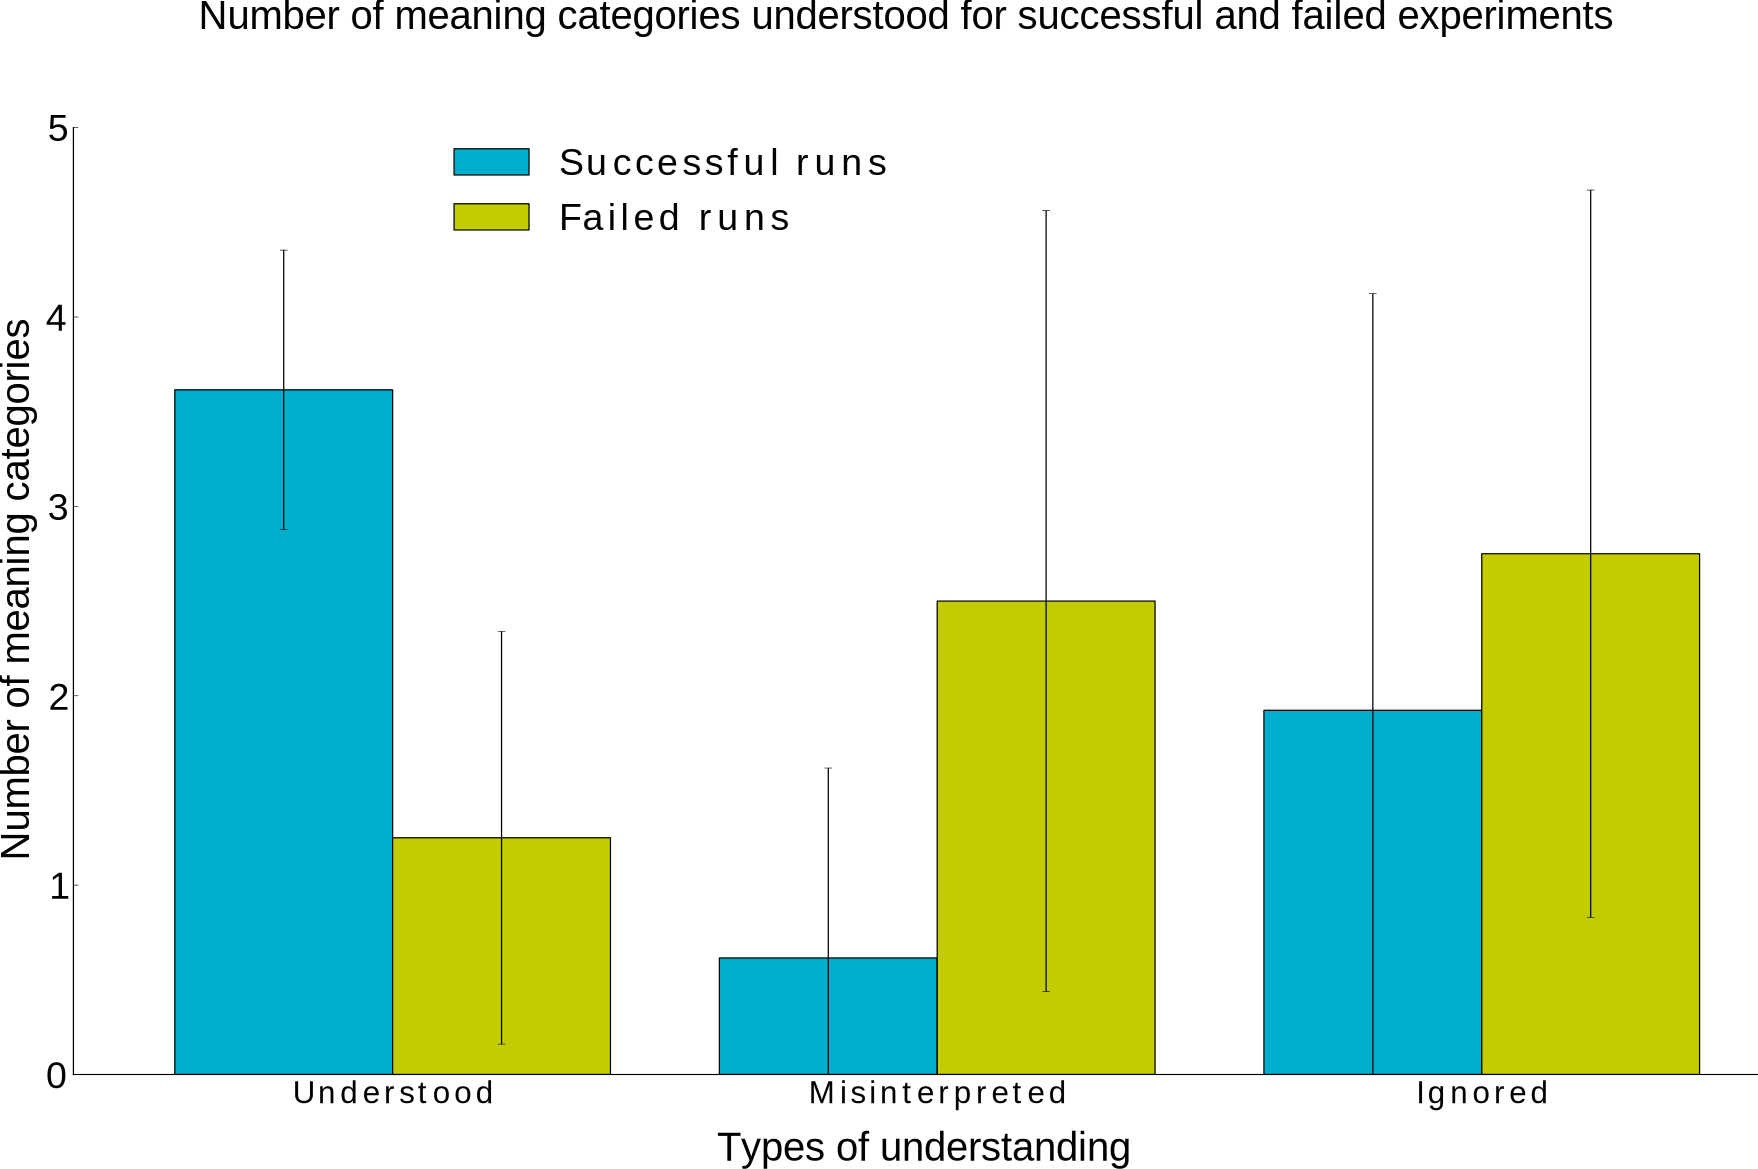
\includegraphics[width=\columnwidth]{\visualspdf/humanexp/meanings/understood_std.pdf}
        \caption{Distribution of meaning categories that were understood, misinterpreted, and ignored by the builders. Average across all builders for successful (blue) and failed (yellow) experiments.}
      \label{fig:types_of_understanding}
    \end{center}
\end{figure}

\begin{figure}[!htbp]
  \begin{center}
      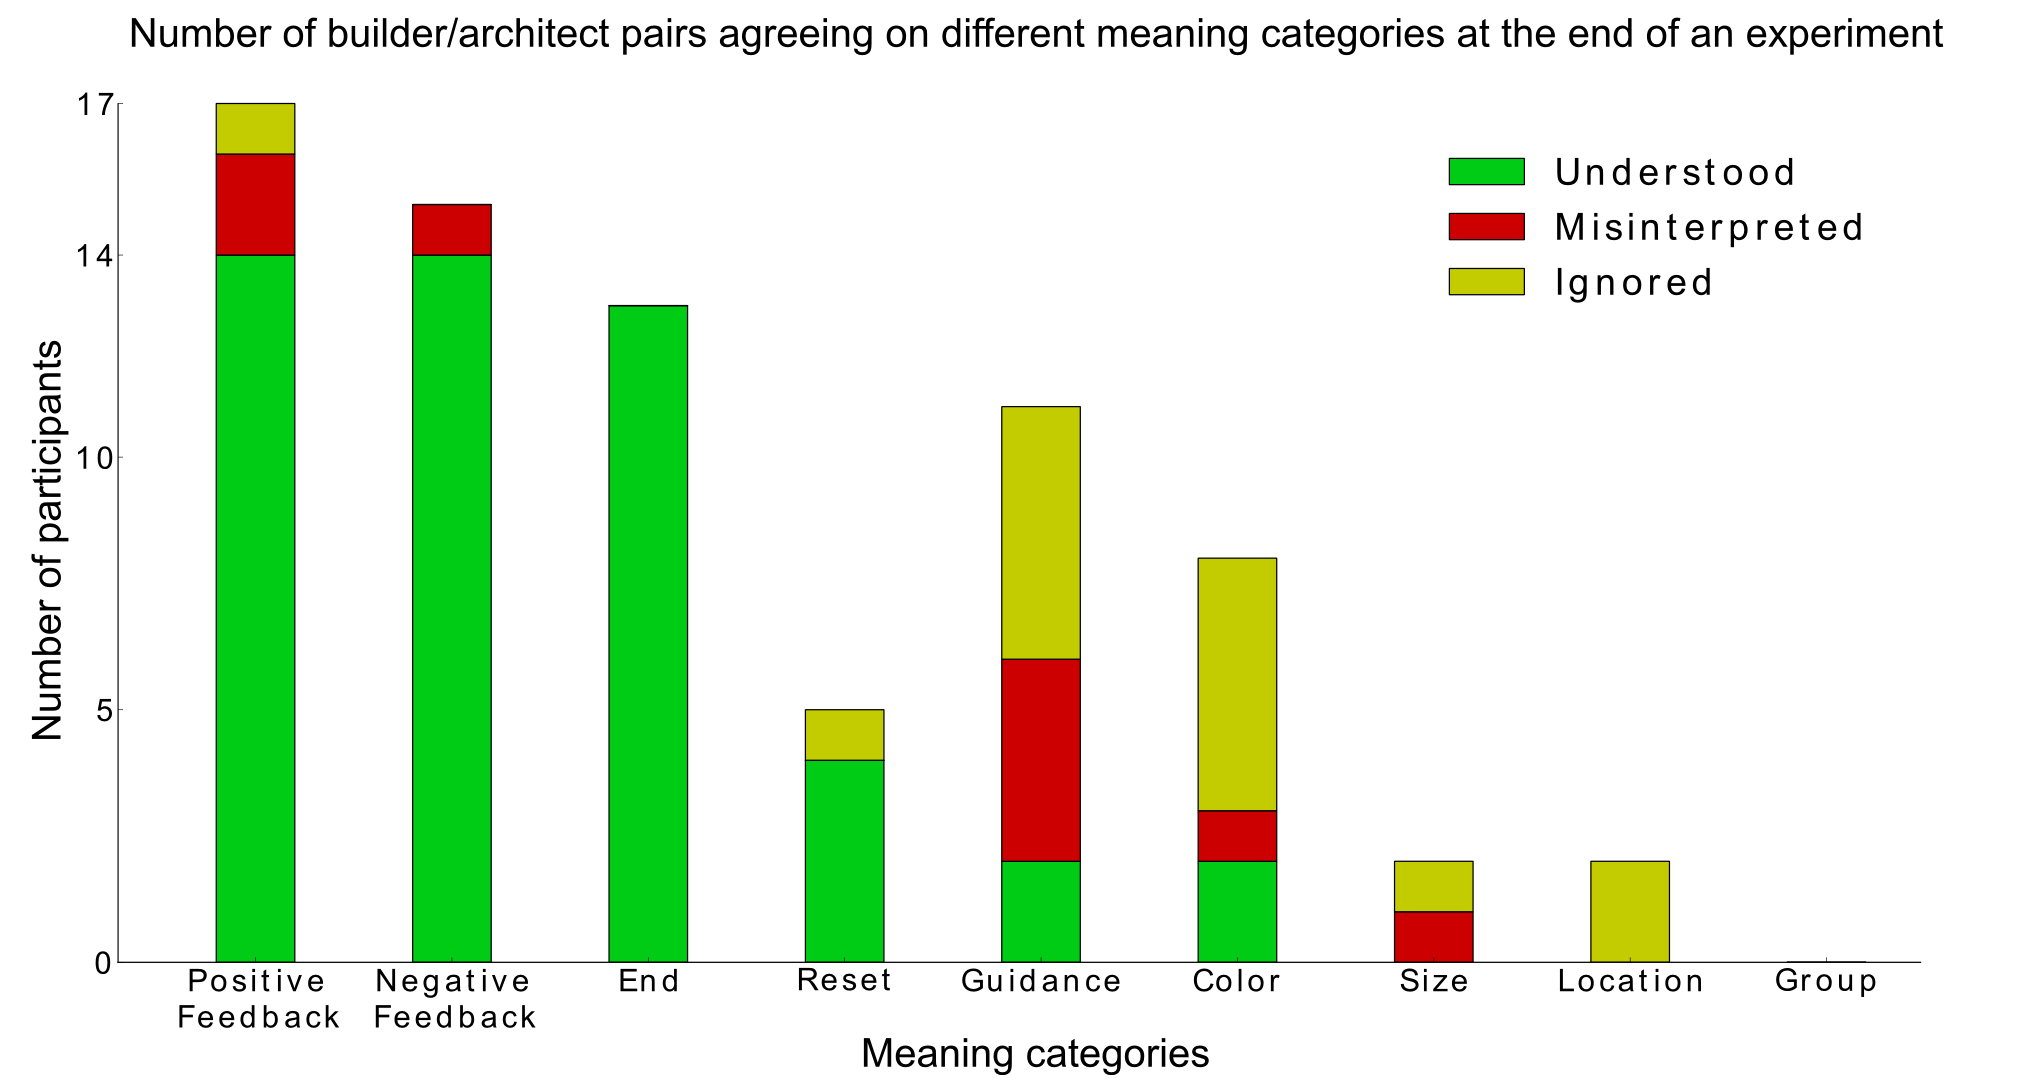
\includegraphics[width=\columnwidth]{\visualspdf/humanexp/meanings/instruction_understood.pdf}
      \caption{Number of builder/architect pairs agreeing or disagreeing on different meaning categories at the end of an experiment.}
    \label{fig:understanding_per_feedback}
    \end{center}
\end{figure}

It seems that even though many different signal meanings are initially considered by the architect, the players agree only on very few specific ones (positive feedback, negative feedback and End). The question of what are the main factors determining which meanings are considered by participants arises. This leads over to the next subsection in which we will consider the builder behavior to explore its role in which signal meanings are considered and in the ultimate outcome of the game.

\subsection{Builder Strategies}
\label{sec:builder}

For the builder, we aimed at identifying common actions across participants in an attempt to quantify the builders' strategies from the video data showing a top-down view of the workspace.
What follows is a description of observations on the builders' behaviors.

We identified two main strategies the builders embarked on (for an overview see Table~\ref{table:builder}). For these two strategies, the builders began by presenting only one block at a time. When they presented several blocks at once throughout the game, they did not seem to embark on a successful strategy.

The most common strategy for builders was to determine one correct brick at a time and to subsequently join it with the already assembled structure (see Figure~\ref{fig:timeline}). Figure~\ref{fig:timeline} is a case example of one game/run of the study in which this strategy is used successfully. The builders in $12$ (five first rounds and their five respective second rounds, one independent single first round, and one second round) of the $17$ runs pursued the same strategy. Only one game (a first round with a successful corresponding second round) of these $12$ failed.

The other strategy was to find all blocks belonging to the target structure. Blocks identified as correct were not joined right away, but in a first step all blocks belonging to the target structure were determined and were then subsequently joined one at a time in a second step. This strategy also involved the presentation of only one block at a time and was eventually pursued by two builders who both started out with a different strategy involving the presentation of multiple blocks. 

One builder initially tried to find which forms belonged to the target structure. Ultimately, he then identified all blocks belonging to the target structure by one at a time dividing all blocks into two groups. This builder played in a second round, for which in its corresponding first round multiple blocks were presented at a time by the builder and the game failed.

Another builder at the beginning tried to elicit a label for either color or form from the architect. In this case, all blocks of one specific color or of one specific shape were presented at a time. This strategy was only pursued by one builder at the beginning of the game, but was not successful and then therefore discontinued in favor of the strategy of finding which blocks belong to the target structure. This builder played in a first round. In the corresponding second round, the builder embarked on the first strategy.

The remaining three builders (in three first rounds) also presented multiple blocks at once but the set of blocks presented did not have any common properties and seemed random. These builders did not have any apparent systematic strategy and their games did not come to a successful end.

 \begin{table}[h]
 \begin{tabular}{p{0.22\columnwidth}|p{0.22\columnwidth}|p{0.12\columnwidth}|p{0.12\columnwidth}|p{0.06\columnwidth}}
%
 \multicolumn{1}{m{0.22\columnwidth}|}{\centering Presentation of blocks} & \multicolumn{1}{m{0.22\columnwidth}|}{\centering Strategy} & \multicolumn{1}{m{0.12\columnwidth}|}{\centering Number of games} & \multicolumn{1}{m{0.12\columnwidth}|}{\centering Successful} & \multicolumn{1}{m{0.06\columnwidth}}{\centering Failed} \\ \hline
%
 \multicolumn{1}{m{0.22\columnwidth}|}{\centering Present one block at a time} & \multicolumn{1}{m{0.22\columnwidth}|}{\centering Find one block and join right away, repeat}                    & \multicolumn{1}{m{0.12\columnwidth}|}{\centering 12}              & \multicolumn{1}{m{0.12\columnwidth}|}{\centering 11}                         & \multicolumn{1}{m{0.06\columnwidth}}{\centering 1}                      \\ \cline{2-5}
% 
  & \multicolumn{1}{m{0.22\columnwidth}|}{\centering Find all blocks belonging to the structure, then start joining} & \multicolumn{1}{m{0.12\columnwidth}|}{\centering 2}                       & \multicolumn{1}{m{0.12\columnwidth}|}{\centering 2}                          & \multicolumn{1}{m{0.06\columnwidth}}{\centering 0} \\ \hline 
 %
 \multicolumn{1}{m{0.22\columnwidth}|}{\centering Present multiple blocks at a time} & \multicolumn{1}{m{0.22\columnwidth}|}{\centering No strategy}                               & \multicolumn{1}{m{0.12\columnwidth}|}{\centering 3}               & \multicolumn{1}{m{0.12\columnwidth}|}{\centering 0}                          & \multicolumn{1}{m{0.06\columnwidth}}{\centering 3}                     
 \end{tabular}
 \caption{}
 \label{table:builder}
 \end{table}

Taking a closer look at the four failed experiments, we find that in one of them, where the builder presented one block at a time, in the end the target construction was almost finished. Architect and builder understood each other, but an early mistake in the position of one block was not signaled by the architect right away. He waited until the rest of the structure was completed and then tried to address the mistake by means of the introduction of a new signal. This new signal was interpreted by the builder as an \emph{End} signal, leading to the end of the game with one block in a position next to the target one. However for the other failed experiments, the structure at the end of the game was far from the target construction and there was no noticeable progress in all three cases.

Whereas, with the current data and analysis, we cannot yet draw any conclusions, still this observation suggests that the way the builders propose next steps and ask for information from the architect is important for the success of the game. Builders seem to build frames and create slots for the architect's input. These frames form the context which shapes the interpretation of the signals. This is similar to how in other cases of asymmetric or restricted communication, as for example in interactions with preverbal infants or in interactions with impaired persons, people provide frames to understand what their interaction partners with their different or limited conversational abilities want to communicate \cite{ochs1979propositions, goodwin1995co}.

\subsection{Additional Observations}

This subsection briefly indicates interesting, additional observations we made with our pilot study, as well as interesting considerations for future work.

First of all, we would like to state that the history of the interaction is crucial for understanding meanings. A person who has not witnessed the course of the interaction, is not able to fill in and complete the task without special instructions. We observe a phase of confusion and negotiation at the beginning of the interactions and after that a completion phase in which signal meanings have been constituted. The latter seems to be characterized by smooth, consistent patterns. In the initial phase of negotiation, we observed instances where the players adapted to their partners by changing the meaning of a button when they noticed the other player understands it differently (cf. Figure~\ref{fig:timeline} in Subsection~\ref{sec:case}). There were for example cases in which the meaning of buttons used to convey a positive or negative feedback reversed.

In contrast, we also observed that some players, both architects and builders, insisted on their strategies, even though the interaction with their respective partner did not work, i.e. they did not agree on any meaning and the task did not progress. Thus, there seem to be leaders and followers in terms of strategies, which could be personality-dependent, but could also manifest their ability to employ a theory of mind.

We also note that when builder and architect switched roles after a first round, their behaviors and performances were influenced (e.g., builder strategies were adopted across rounds). If a second round was systematically part of the experimental procedure, it would be interesting to see whether participants succeed faster in the second game they play with reversed roles and if they adopt similar strategies.

Another interesting aspect concerns timing, not only at which points in time the architect gives feedback and instructions, but also the interplay between the builder's and the architect's actions. The rhythm of the interaction partners' actions might be an important low-level feature in determining whether a certain signal means positive or negative feedback.

While the above points are highly relevant and worth investigating, their detailed examination is beyond the scope of this work.

\paragraph{Meaning switches and reset} 

During the experiment, we noticed some participants were misinterpreting a \emph{Positive feedback} as a \emph{Negative feedback} (and reversely), but most of the time they were able to detect and correct this misunderstanding. In few cases, it was the architect that inverted the meaning of the signals but in most cases it was the builder that had to reinterpret the signals, often after a \emph{Reset} instruction from the architect. The data we collected are not detailed enough for a fine-grained temporal analysis but we were able to count the number of feedback interpretation switches per run. In 5 out of 14 successful games (see Figure~\ref{fig:feedback_switch_enhanced}) the architect or the builder changed his use or interpretation of signals between positive and negative feedback.

\begin{figure}[!htbp]
  \begin{center}
      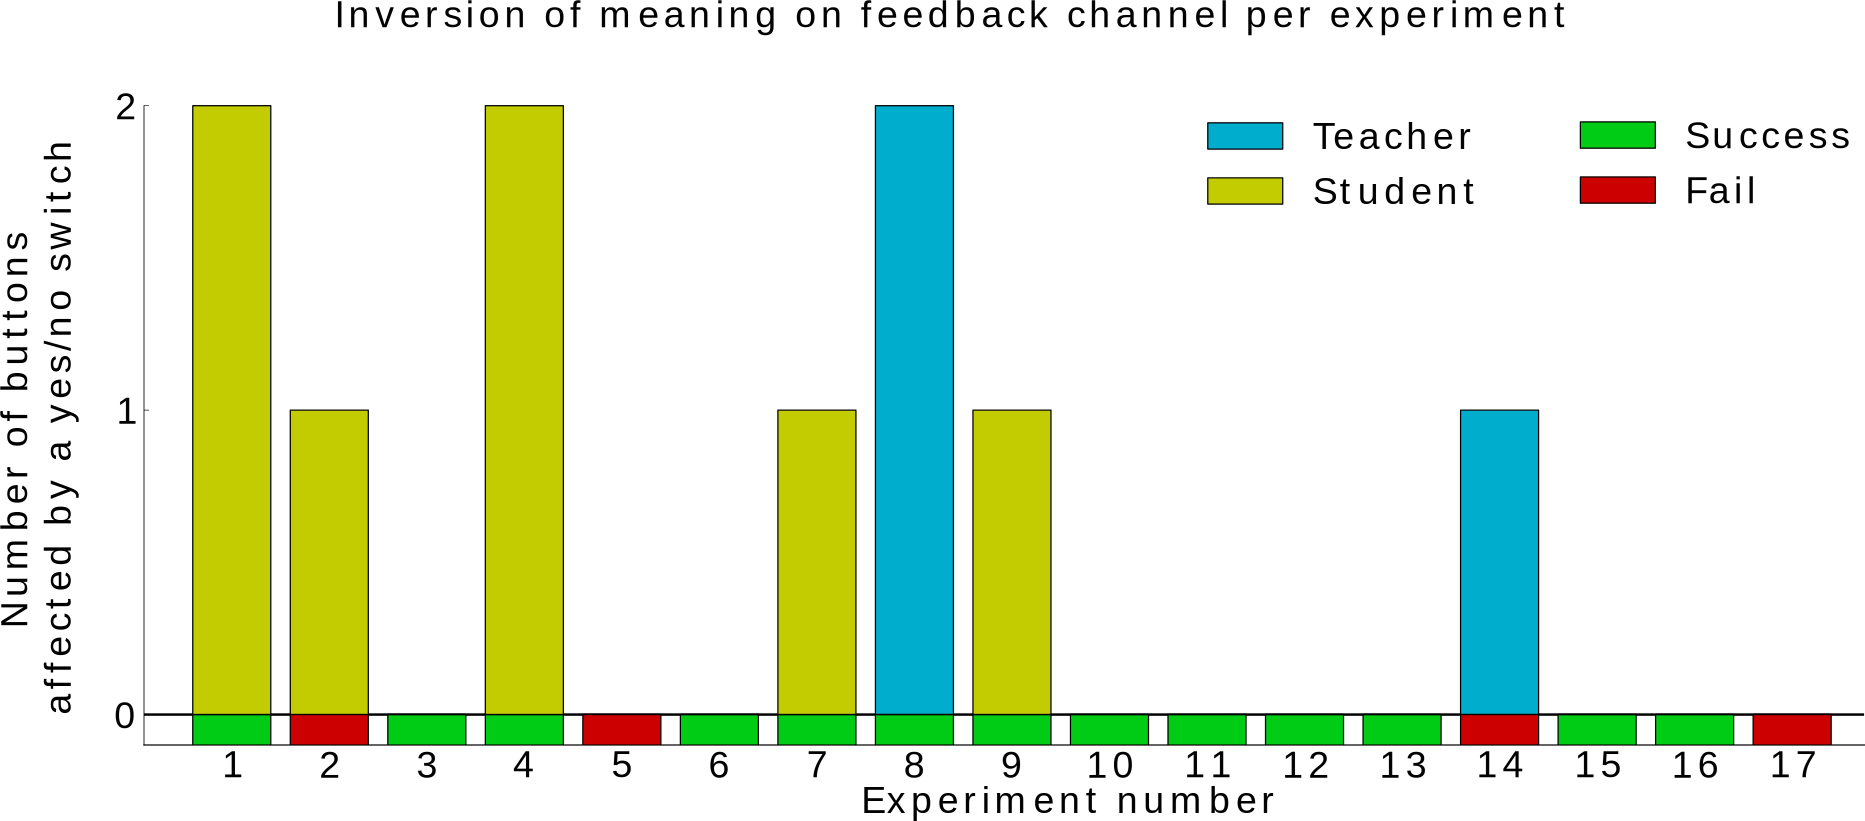
\includegraphics[width=\columnwidth]{\visualspdf/humanexp/meanings/inversion_meaning.pdf}
      \caption{Number of signals whose meanings switch between positive and negative feedback during the experiment. In blue, cases where the architect decides to change the meaning of a button from one feedback type to the other. In yellow, cases where the builder changes his/her interpretation of a signal. The colored bar on the bottom indicates if the experiment was successful or not.}
    \label{fig:feedback_switch_enhanced}
    \end{center}
\end{figure}


\paragraph{Context dependent meaning} 

In several cases the architect pressed all buttons to signify a salient event. This event was either perceived as a \emph{Reset} instruction if the builder felt lost or an \emph{End} instruction if the builder felt confident about his/her understanding of the previous interaction sequences. This is illustrated in figure~\ref{fig:timeline}, where at $t=200 s$, as players already tried for several iteration with no success, the architect presses all buttons to signify a \emph{Reset}. After this \emph{Reset}, a new set of symbols is used by the architect which is well understood. Finally, to signify that the construction is finished, the architect presses again all buttons simultaneously now with the intended meaning that the task is completed. As the interaction was going well, this signal was understood as a \emph{End} signal by the builder and the experiment goes to a successful end.

As detailed earlier one of the experiment failed even if the in the end the target construction was almost finished. Architect and builder understood each other, but an early mistake in the position of one block was not signaled by the architect right away. He waited until the rest of the structure was completed and then tried to address the mistake by means of the introduction of a new signal. Given the context (the interaction was smooth and participants understood each other), the introduction of this new signal was interpreted by the builder as an \emph{End} signal, leading to the end of the game with one block in a position next to the target one.

\paragraph{Timing} 

Figure~\ref{fig:timeline} contains information on which signal the architect sends to the builder at which point in time as well at its alignment with the construction progress. Such information allow to analyse the timing and interplay of interaction at both a micro and macro scale.

\paragraph{Confirmation bias} 

Some builders were affected by the confirmation bias which is defined as \textit{``the seeking or interpreting of evidence in ways that are partial to existing beliefs, expectations, or a hypothesis in hand''} \cite{nickerson1998confirmation}. While mistaking negative feedback for positive feedback, participants were progressing far in a wrong direction, even if the signal would seem contradictory for an outside observer. It was difficult for some users to re-assess their belief, they better thought the architect was mistaking or were pursuing in a very improbable direction. Few builders were able to overcome the confirmation bias problem by themselves, leading either to a failed experiment or needed the architect to produce a salient event to reset the experiment. With the recorded data, it is unfortunately not possible to quantify this phenomenon even if the figure~\ref{fig:feedback_switch_enhanced} may provide useful information.

\paragraph{Workspace} 

From our video recording, we observed that some builders (9 out of 17) cleaned their workspace in the beginning of the experiment, such that no block is remains visible. They then tried to maintain a clean workspace during the game, giving them a presentation space, where they could propose blocks in an unambiguous way. Another strategy was pursued by eight builders who from the beginning kept all blocks on the workspace and therewith enabled the architect to witness the process of choice of block. Of these eight builders, three neatly ordered and aligned their blocks on the workspace and proposed one block at a time by pointing to it. The remaining five builders did not order or align the blocks in any way. These participants opened up a workspace inside the overall workspace (i.e., proposing blocks in-between or next to the rest).

% \begin{itemize}
% \item clean workspace used as presentation space (9)
% \item all blocks in view (8) (nicely aligned (3), or not aligned (5))
% \end{itemize}

\paragraph{Propositions} 

Essentially the task consisted in two subtasks, finding correct blocks and joining them. For this, participants proposed blocks and positions of blocks in different ways. For proposing blocks in search for a correct one, builders ``present'' blocks by placing them alone on the workspace or in a separate sub-workspace, they point to the block they wish to receive feedback about, or they lift the respective block to highlight it.

% \begin{itemize}
% \item present
% \item point
% \item lift
% \end{itemize}

To find at which position a specific block is correctly joined with others, the propositions differ in the level of accuracy and precision of the proposed position. Some builders begin with bumping two blocks together to receive feedback about if they should be joined at all. In some cases the respective block is placed above, below, on the right or on the left of a structure to receive course feedback about the location of the correct position. Another way of presentation is to continuously move the respective block around the structure with expected positive feedback when the correct position is reached. Some builders discretely test or propose positions on the way around the structure by only pausing, joining blocks half way, or fully joining the blocks at each possible position.

% \begin{itemize}
% \item bump
% \item order (bottom to top)
% \item right, left, above, below
% \item continuously move around the structure
% \item discretely stop at each position or join half-way
% \item join at each possible position
% \end{itemize}

%%%%%%%%%%%%%%%%%%%%%%%%%%%%%%%%%%%%%%%%%%%%%%
%%%%%%%%%%%%%%%%%%%%%%%%%%%%%%%%%%%%%%%%%%%%%%
%%%%%%%%%%%%%%%%%%%%%%%%%%%%%%%%%%%%%%%%%%%%%%
%%%%%%%%%%%%%%%%%%%%%%%%%%%%%%%%%%%%%%%%%%%%%%
%%%%%%%%%%%%%%%%%%%%%%%%%%%%%%%%%%%%%%%%%%%%%%
\section{Lessons Learned}

We presented a new experimental method which allows to study important aspects of human communication with high relevance to human-robot interaction. We show that two players that never had a chance to interact by the means of a restricted interface before were able to communicate and act upon communicative acts whose meanings were never explicitly negotiated between interaction partners. What can we learn from the experiments? How can it be used for human-robot interaction?

We first link our experiment with the concept of interaction frame defined in introduction (chapter~\ref{chapter:introduction}). We then describe the main strategy used by our participants. We highlight the active role of the builder in creating slots for the architect to provide information. And further identify the main strategy used to learn the meanings of button presses, which consist of generating interpretation hypothesis and trying to validate or discard them through further interactions. 

% Finally, and based on those observations, we start defining the problem of learning from unlabeled interaction frame in more concrete terms.

\subsection{Use of interaction frames}
\label{chapter:humanexperiment:frames}

The experimental setup setup described above is less constrained than our challenge of \emph{learning fro unlabeled interaction frames} defined previously. As a reminder this problem assume the interaction frames associated to the interaction between the robot and the human is known and only the mapping between signal of the teacher and their meaning is unknown. Knowing the interaction frame, include knowing: \begin{inparaenum}[(a)] \item the set of possible meanings the human can refer to, \item the details and timing of the interaction, and \item the constraints that apply on the possible tasks. \end{inparaenum}

In the human-human experiment described in this chapter, the interaction frame is not defined in advance. The meanings associated to the button events are not constrained to belong to a finite set, and the details and timing of the interaction, i.e. the protocol, are also undefined at start. Only the context in which the interaction takes place is provided to both participant, which is to build a flat construction which does not necessarily contain all available blocks.

The first interesting fact is that, while all of participants thought the problem impossible to solve, most of them were able to successfully cooperate under restricted and asymmetric interaction.

The second interesting fact is that users seemed to rely on ``usual'' interaction frames to make sense of the interaction (cf figure~\ref{fig:types_of_feedback}). Especially, participants came up with strategies involving both the details and timing of the interaction and the possible meanings associated to the button events.In the following two subsections, we will highlight the following observations: 

\begin{itemize}

\item the timing and alignment between both participants quickly converged. Especially the builder seemed to be the leader in the construction of the interaction protocol. With his/her propositions of blocks and positions, the builder provides frames in which he/she creates slots for the architect to provide information.

\item the architects and the builders considered only a limited number of meaning types; among which only positive and negative feedback was considered by all participant. Builders seem to rely on the assumption that the signal observed would belong to one of this categories. He then relied on interpretation hypothesis with respect to both the task (i.e. the possible construction) and the meaning of the signals. By testing several combination of task and signal's meaning, the builder was able to identify the correct signal to meaning mapping most often leading to a success in the construction task.

\end{itemize}

\subsection{Slots of interaction}

Signals' meanings is co-constructed by the interaction partners, but the builder's actions seems to play an important role in the understanding of signals. With his/her propositions of blocks and positions, the builder provides frames in which he/she creates slots for the architect to provide information. And thus the builder's created frames constrain the meaning of the architect's input to a large extent. 

For example, by cleaning the workspace of all blocks and presenting new blocks one at a time, the builder influence the architect to provide a signal whose meaning can be: ``this block belongs/does not belong to the construction'' or ``this block is blue/red/yellow'' for example. This way the builder additionally impose the timing of the interaction, e.g. a turn taking social behavior where the builders propose a new block and waits for a signal from the architect. As a result, the builders is now faced with a similar problem than our problem of \emph{learning from unlabeled interaction frames}, where the meanings are limited to a limited set known from both partners, and the association between world's event (e.g. movement of cubes) and instruction signals is known. However the particular meaning of the button presses inside each frame is still to identify, e.g. whether the observed signal means the block belongs or does not belong to the final structure.

This behavior also been found in asymmetric and restricted interactions with interaction partners with limited communicational abilities, as for example preverbal infants or impaired persons \cite{ochs1979propositions, goodwin1995co}. 

Therefore, it might be interesting to consider similar mechanism of proposition in a learning robot could be a means to elicit appropriate signals from a human tutor in HRI \cite{cakmak2012designing,vollmer2014robots,cangelosi2010integration}. And this even if the interaction protocol is not not explicitly given to the human tutor in advance. These interesting directions are not the subject of this thesis, and in our experiments we will assume the human teacher is aware of the interaction frame. It is only in chapter~\ref{chapter:limitations:framehypothesis} that we soften this assumption, assuming a finite set of possible interaction frames is available.

\subsection{Interpretation hypothesis}
\label{chapter:humanexperiment:interpretationhypothesis}

Both builder and architect have preconceptions of what interaction frames the other player is likely to understand, trying to use or interpret signals with respect to those frames. The ``feedback frame'' seems the most commonly thought about and the easiest to understand in the context of our experiment.

Humans are capable of solving the kind of communication problem robots can have with humans. We have observed that humans can solve such restricted asymmetric interaction problems by projecting the interaction into different common interaction frames and selecting the one that is more coherent with the history of interaction. In this setup such an interaction frame provides information about many properties of the interaction including for example \begin{inparaenum}[(a)]  \item a context (e.g. building something with a limited number of blocks and specific constraints (on a table, flat, \ldots)) which represents task constraints that are specified in advance, and \item a set of possible frames (e.g. feedback, guidance, references to colors or shapes), which we acquired from our experience interacting with others. \end{inparaenum}

Based on such observations, by replacing the builder by an artificial agent (e.g. a robot), we can aim at constructing robots capable of learning a task from human instructions without programming them in advance to understand the human communicative acts and without pre-programming a specific rigid interaction protocol. To do so, we should inform the robot about the context of the interaction, i.e. some task contraints, and equip the robot with one or several interaction frames on which it can rely on to find a coherence between the interaction history with the human, a particlar frame, and a particlar task. We formalize this idea in next section.

, with a \emph{Reset} and an \emph{End} instructions more frequently considered than guidance, color, or size related instructions.
